
%\setcounter{chapter}{13}
\chapter{Backpropagation}\label{chapter:backpropagation}

\index{Backpropagation}
\section{Introduction}
A key idea of neural nets is to decompose computation into a series of layers. In this chapter we will think of layers as modular blocks that can be chained together into a \index{Computation graph}\textbf{computation graph}. \Fig{\ref{fig:backpropagation:simple_MLP}} shows the computation graph for the two-layer multilayer perceptron (MLP) from \chap{\ref{chapter:neural_nets}}.

\vspace{-0.2cm}
\begin{figure}[h]
\begin{minipage}{.23\textwidth}
\centering
\begin{tikzpicture}[>=spaced latex]
\draw [thick] (0,-0.75) circle [radius=0.2] node[label={$\mathbf{x}$}] at (0,0.85) {};
\draw [thick] (0,0.1) node {$\vdots$};
\draw [thick] (0,0.75) circle [radius=0.2];

\draw [thick,dotted] (0.33,-1.2)  .. controls (0.43,-1.05) .. (0.43,-0.9);
\draw (0.4,-1.45) node {$\mathbf{W}_1$};

\draw [thick] [nn_edge] (0.2,-0.75) -- (0.8,-0.1);
\draw [thick] [nn_edge] (0.2,-0.75) -- (0.8,-0.75);
\draw [thick] [nn_edge] (0.2,-0.75) -- (0.8,0.75);
\draw [thick] [nn_edge] (0.2,-0.1) -- (0.8,-0.75);
\draw [thick] [nn_edge] (0.2,0.0) -- (0.8,0.0);
\draw [thick] [nn_edge] (0.2,0.1) -- (0.8,0.75);
\draw [thick] [nn_edge] (0.2,0.75) -- (0.8,0.75);
\draw [thick] [nn_edge] (0.2,0.75) -- (0.8,-0.75);
\draw [thick] [nn_edge] (0.2,0.75) -- (0.8,0.1);
\draw [thick, fill=gray_neuron] (1,0.75) circle [radius=0.2]  node[label={$\mathbf{z}$}] at (1.0,0.85) {};
\draw [thick] (1,0.1) node {$\vdots$};
\draw [thick, fill=gray_neuron] (1,-0.75) circle [radius=0.2];
\draw [thick] [nn_edge] (1.2,0.75) -- (1.8,0.75);
\draw [thick] [nn_edge] (1.2,0.0) -- (1.8,0.0);
\draw [thick] [nn_edge] (1.2,-0.75) -- (1.8,-0.75);
\draw [thick, fill=gray_neuron] (1,0.75) circle [radius=0.2]  node[label={$\mathbf{h}$}] at (2.0,0.85) {};
\draw [thick, fill=gray_neuron] (2.0,0.75) circle [radius=0.2];
\draw [thick] (2.0,0.1) node {$\vdots$};
\draw [thick, fill=gray_neuron] (2.0,-0.75) circle [radius=0.2];

\draw [thick,dotted] (2.33,-1.2)  .. controls (2.43,-1.05) .. (2.43,-0.9);
\draw (2.4,-1.45) node {$\mathbf{W}_2$};

\draw [thick] [nn_edge] (2.2,-0.75) -- (2.8,-0.75);
\draw [thick] [nn_edge] (2.2,-0.75) -- (2.8,0.75);
\draw [thick] [nn_edge] (2.2,-0.75) -- (2.8,0.0);
\draw [thick] [nn_edge] (2.2,-0.1) -- (2.8,-0.75);
\draw [thick] [nn_edge] (2.2,0.0) -- (2.8,0.0);
\draw [thick] [nn_edge] (2.2,0.1) -- (2.8,0.75);
\draw [thick] [nn_edge] (2.2,0.75) -- (2.8,0.75);
\draw [thick] [nn_edge] (2.2,0.75) -- (2.8,-0.75);
\draw [thick] [nn_edge] (2.2,0.75) -- (2.8,0.0);
\draw [thick] (3.0,-0.75) circle [radius=0.2] node[label={$\mathbf{y}$}] at (3.0,0.8) {};
\draw [thick] (3.0,0.1)  node {$\vdots$};
\draw [thick] (3.0,0.75) circle [radius=0.2];
\end{tikzpicture}
\end{minipage}
%
%
\begin{minipage}{0.77\textwidth}
\centering
\def\layerwidth{1.3}
\begin{tikzpicture}[
cblock/.style={
draw,
fill=comp_graph_node_bcolor,
rectangle, 
inner sep=1.5mm,
minimum width=\layerwidth*0.9 cm,
minimum height=\layerwidth*0.5*0.9 cm,
font=\footnotesize}]
%
\draw [thick] [comp_graph_edge] (\layerwidth*0.5,0) -- (\layerwidth,0);
%\draw (0,0) rectangle ++(1,1);
\draw (\layerwidth*1.5,0) node [cblock] {\texttt{linear}};
\draw [thick] [comp_graph_edge] (\layerwidth*2,0) -- (\layerwidth*3,0);
\draw (\layerwidth*3.5,0) node [cblock] {\texttt{relu}};
\draw [thick] [comp_graph_edge] (\layerwidth*4,0) -- (\layerwidth*5,0);
\draw (\layerwidth*5.5,0) node [cblock] {\texttt{linear}};
\draw [thick] [comp_graph_edge] (\layerwidth*6,0) -- (\layerwidth*6.25,0);

\draw (\layerwidth*0.5,0) node [fill=comp_graph_data_bcolor] {$\mathbf{x}$};
\draw (\layerwidth*2.5,0) node [fill=comp_graph_data_bcolor] {$\mathbf{z}$};
\draw (\layerwidth*4.5,0) node [fill=comp_graph_data_bcolor] {$\mathbf{h}$};
\draw (\layerwidth*6.5,0) node [fill=comp_graph_data_bcolor] {$\hat{\mathbf{y}}$};

\draw (-1,0) node {$\iff$};
\end{tikzpicture}
\end{minipage}
\caption{In this chapter we will visualize neural nets as a sequence of layers, which we call a computation graph.}
\label{fig:backpropagation:simple_MLP}
\end{figure}
\vspace{-0.2cm}

Each {\setlength{\fboxsep}{2pt}\colorbox{comp_graph_node_bcolor}{layer}} takes in some inputs and transforms them into some outputs. We call this the $\texttt{forward}$ pass through the layer. If the layer has parameters, we will consider the parameters to be an \textit{input} to a parameter-free transformation:
\begin{align}
    \xout &= f(\xin,\theta)
\end{align}
Graphically, we will depict the forward operation of a layer like shown below (\fig{\ref{fig:backpropagation:mod_block_forward}}).
\vspace{-0.2cm}
\begin{figure}[h]
\centerline{
\begin{tikzpicture}%[>=spaced latex]
%
\def\layerwidth{1.8}
%
\draw [thick] [comp_graph_edge] (\layerwidth*0.6,-0.35) -- (\layerwidth,-0.35);
\draw [thick] (\layerwidth*0.6,-0.75) -- (\layerwidth*0.6,-0.35);
\draw [thick] [comp_graph_edge] (\layerwidth*0.5,0) -- (\layerwidth,0);
\draw (\layerwidth*1.5,0) node [fill=comp_graph_node_bcolor,draw, inner sep=2mm, minimum height=1.3cm] {$f(\xin, \theta)$};
\draw [thick] [comp_graph_edge] (\layerwidth*2,0) -- (\layerwidth*2.4,0);
%
\draw (\layerwidth*0.6,-0.95) node [fill=white] {$\theta$};
\draw (\layerwidth*0.4,0) node [fill=comp_graph_data_bcolor] {$\xin$};
\draw (\layerwidth*2.65,0) node [fill=comp_graph_data_bcolor] {$\xout$};
\draw (\layerwidth*1.5,1) node {\texttt{forward}};
%
\end{tikzpicture}
}
\caption{Forward operation of a neural net layer.}
\label{fig:backpropagation:mod_block_forward}
\end{figure}
\vspace{-0.2cm}

% \begin{figure}[h]
% \centering
% \begin{tikzpicture}%[>=spaced latex]
% %
% \def\layerheight{1.0}

% \draw [thick] [comp_graph_edge] (0,0) -- (0,\layerheight);
% %\draw (0,0) rectangle ++(1,1);
% \draw (0,\layerheight*1.5) node [fill=comp_graph_node_bcolor,draw, inner sep=2mm] {$f(\xin)$};
% \draw [thick] [comp_graph_edge] (0,\layerheight*2) -- (0,\layerheight*3);

% \draw (0,\layerheight*0.4) node [fill=comp_graph_data_bcolor] {$\xin$};
% \draw (0,\layerheight*2.4) node [fill=comp_graph_data_bcolor] {$\xout$};

% \end{tikzpicture}
% \label{fig:backpropagation:mod_block}
% \end{figure}

% \begin{figure}[h]
%     \centering
%     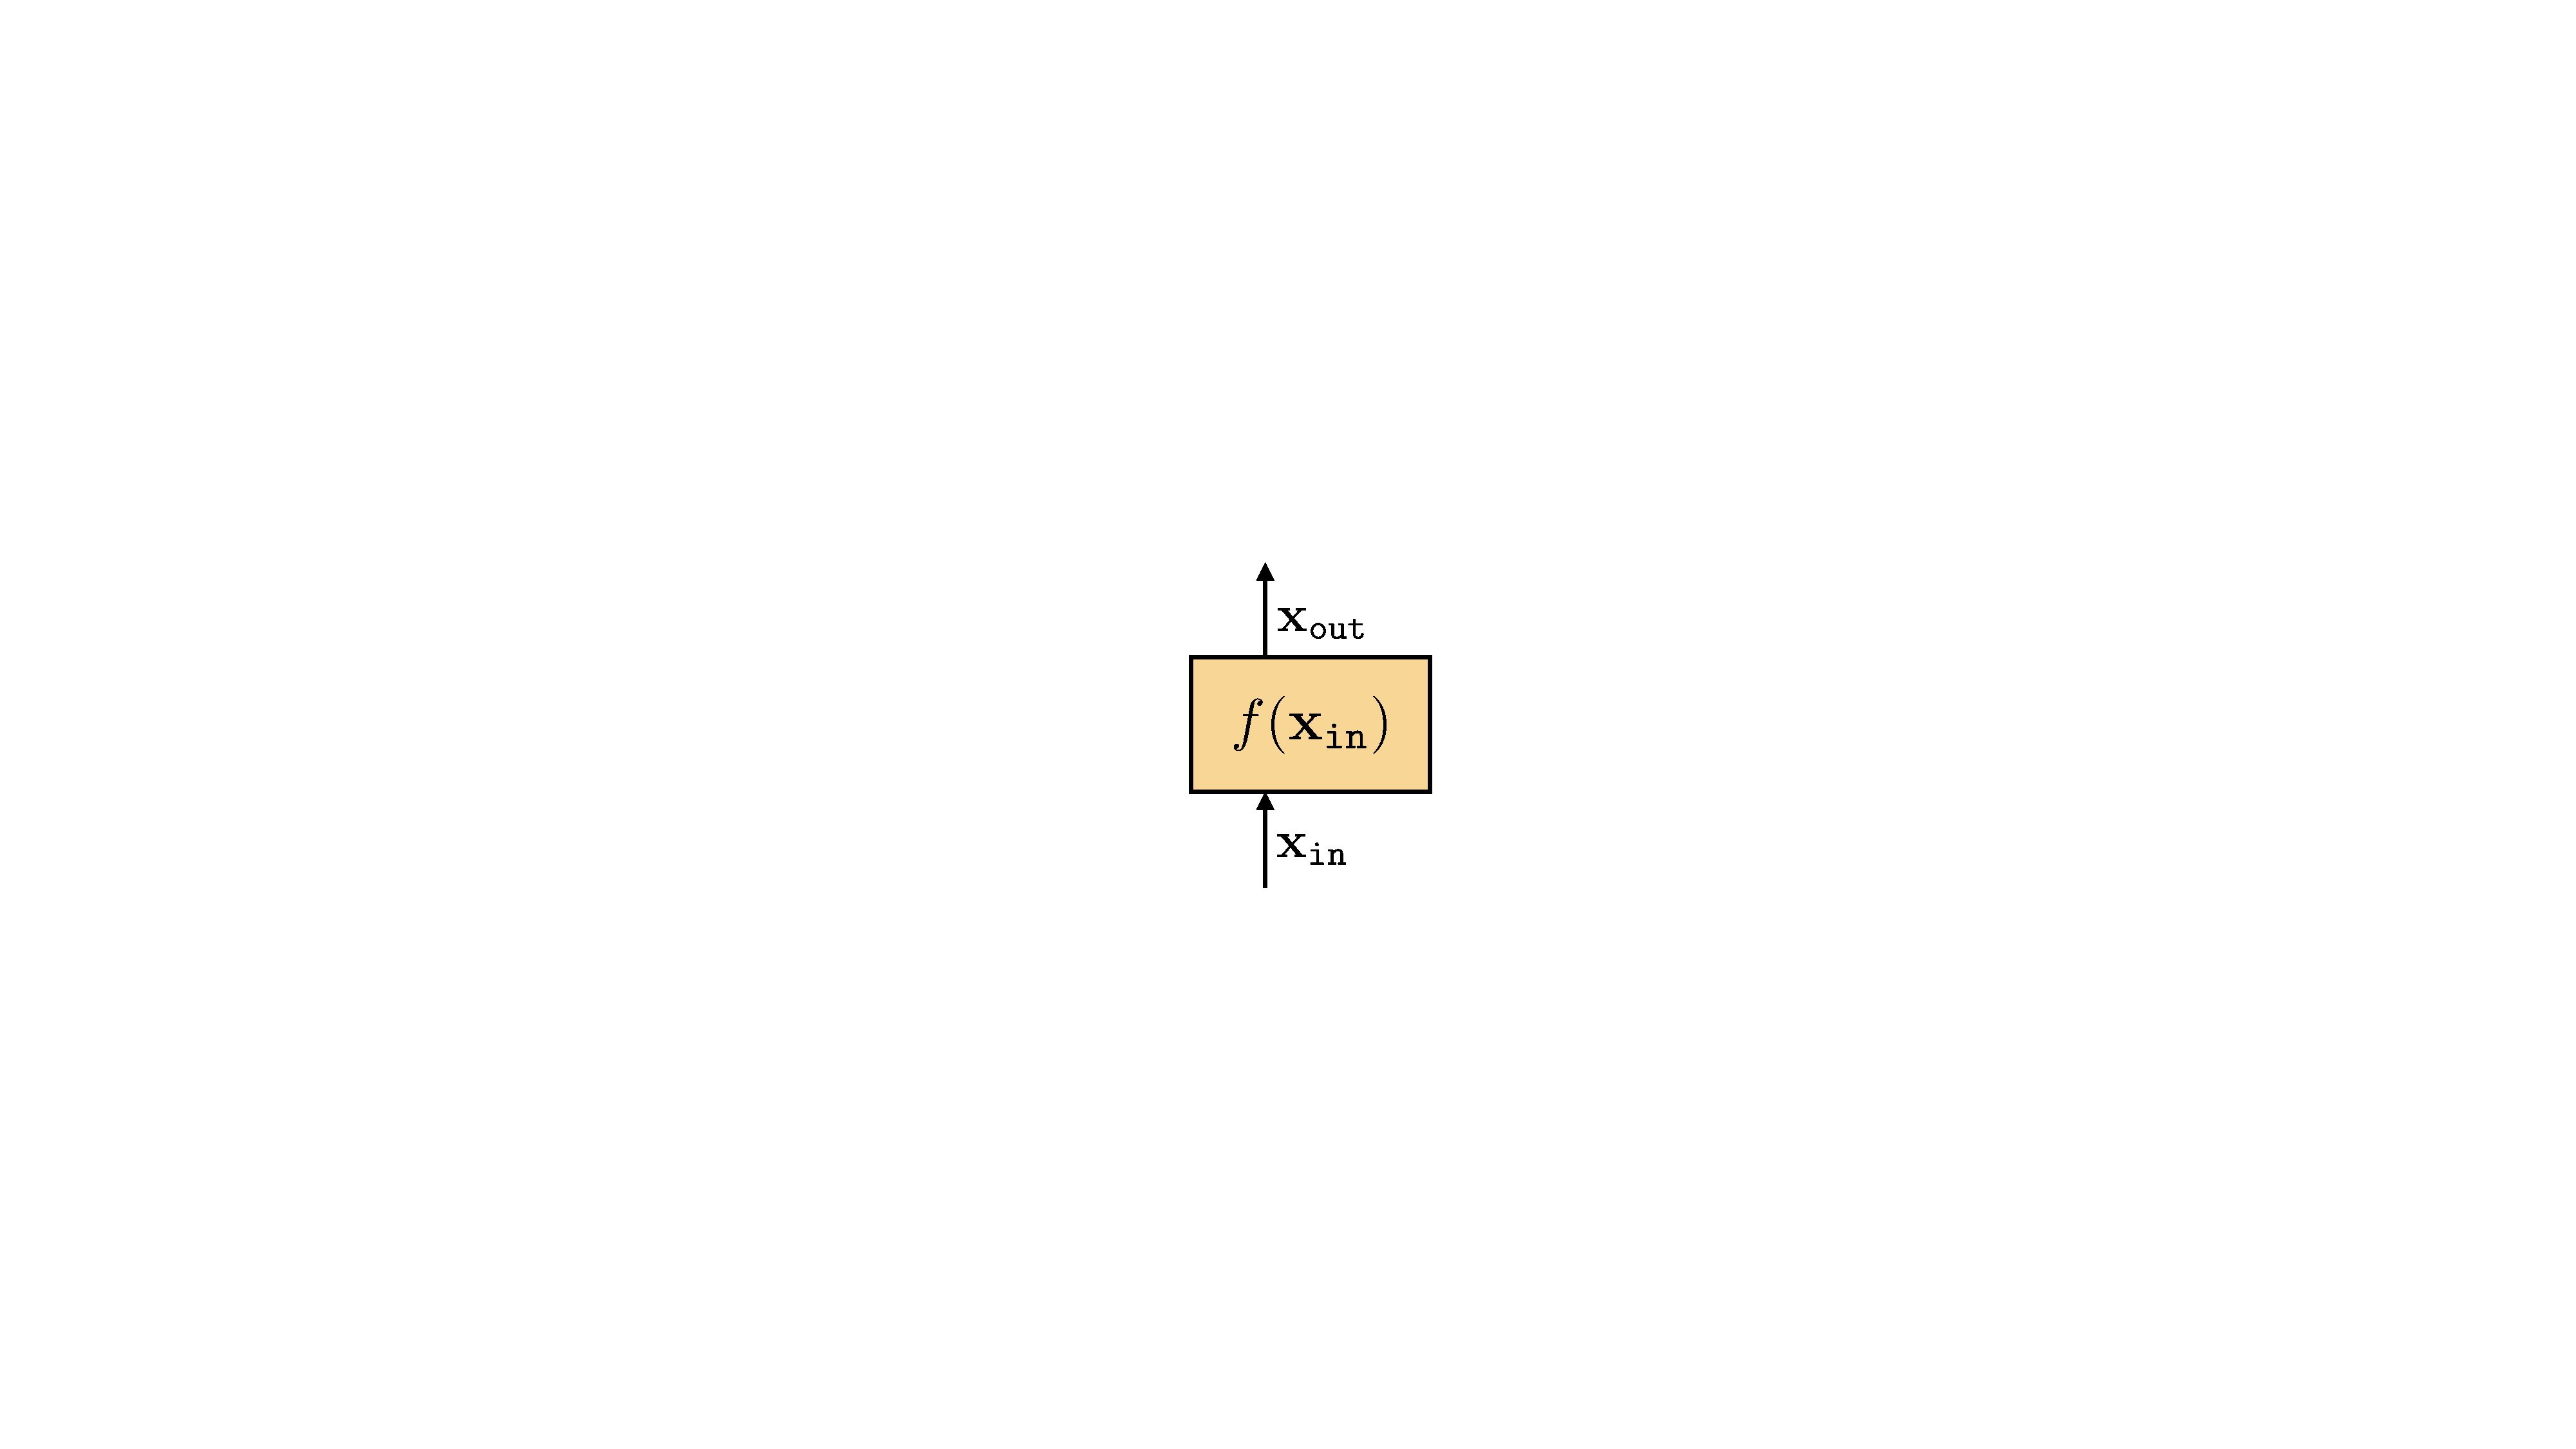
\includegraphics[width=0.18\linewidth]{./figures/backpropagation/mod_block.pdf}
%     \label{fig:mod_block}
% \end{figure}

%A graph of computational blocks like this is called a \textbf{computation graph}.

The learning problem is to find the parameters {\setlength{\fboxsep}{2pt}\colorbox{comp_graph_param_bcolor}{$\theta$}} that achieve a desired mapping. Usually we will solve this problem via gradient descent. The question of this chapter is, how do we compute the gradients?
\marginnote{We will use the color \raisebox{1mm}{\colorbox{comp_graph_param_bcolor}{\makebox(0,0){}}} to indicate \textit{free} parameters, which are set via learning and are not the result of any other processing.}[-1.9cm]
%These parameters, along with the input training data, are the leaves in the computation graph.

\textbf{Backpropagation} is an algorithm that efficiently calculates the gradient of the loss with respect to each and every parameter in a computation graph. It relies on a special new operation, called \texttt{backward} that, just like \texttt{forward}, can be defined for each layer, and acts in isolation from the rest of the graph. But first, before we get to defining \texttt{backward}, we will build up some intuition about the key trick backpropagation will exploit.

\section{The Trick of Backpropagation: Reuse of Computation}

To start, we will consider a simple computation graph that is a chain of functions $f_L \circ f_{L-1} \circ \cdots f_2 \circ f_1$, with each function $f_l$ parameterized by $\theta_l$.\marginnote{Such a computation graph could represent an MLP, for example, which we will see in the next section.}[-0.4cm] We aim to optimize the parameters with respect to a loss function $\mathcal{L}$. The loss can be treated as another node in our computation graph, which takes in $\mathbf{x}_L$ (the output of $f_L$) and outputs a scalar $J$, the loss. This computation graph appears as follows (\fig{\ref{fig:backpropagation:composed_modules}}).
\begin{figure}[h]
    \centerline{
    \def\layerwidth{1.2}
    \begin{tikzpicture}[
    cblock/.style={
    draw,
    fill=comp_graph_node_bcolor,
    rectangle, 
    inner sep=1.5mm,
    minimum width=\layerwidth*0.9 cm,
    minimum height=\layerwidth*0.75*0.9 cm}]
    %
    %
    % draw f nodes
    \def\fnames {{"$f_0$","$f_1$","$f_2$","$f_{L-1}$","$f_L$"}}
    \foreach \x in {1,2,3,4} {
        \pgfmathparse{\fnames[\x]};
        \draw ($(\layerwidth*2*\x-\layerwidth+\layerwidth*0.5,0)$) node [cblock] {\pgfmathresult};
    }
    % draw data arrows
    \draw [thick] [comp_graph_edge] (\layerwidth*0.5,0) -- (\layerwidth,0);
    \foreach \x in {1,2,3,4} {
        % data arrow
        \draw [thick] [comp_graph_edge] (\layerwidth*2*\x,0) -- (\layerwidth*2*\x+\layerwidth,0);
    }
    \draw [thick] [comp_graph_edge] (\layerwidth*10,0) -- (\layerwidth*10.25,0);
    %
    % draw param arrows
    \foreach \x in {0,1,2,3} {
        \draw [thick] [comp_graph_edge] (\layerwidth*2*\x+\layerwidth*0.6,-0.35) -- (\layerwidth*2*\x+\layerwidth,-0.35);
        \draw [thick] (\layerwidth*2*\x+\layerwidth*0.6,-0.75) -- (\layerwidth*2*\x+\layerwidth*0.6,-0.35);
    }
    %
    % draw data and params
    \def\datanames {{"$\mathbf{x}_0$","$\mathbf{x}_1$","$\cdots$","$\mathbf{x}_{L-1}$","$\mathbf{x}_L$"}}
    \def\paramnames {{"$\theta_1$","$\theta_2$","$\theta_{L-1}$","$\theta_{L}$"}}
    \foreach \x in {0,1,2,3,4} {
        \pgfmathparse{\datanames[\x]};
        \draw ($(\layerwidth*2*\x+\layerwidth*0.5,0)$) node [fill=comp_graph_data_bcolor] {\pgfmathresult};
        %
    };
    \foreach \x in {0,1,2,3} {
        \pgfmathparse{\paramnames[\x]};
        \draw ($(\layerwidth*2*\x+\layerwidth*0.5,-0.95)$) node [fill=comp_graph_param_bcolor] {\pgfmathresult};
    };
    %
    % loss node
    \draw (\layerwidth*9.5,0) node [cblock, fill=comp_graph_loss_node_bcolor] {$\mathcal{L}$};
    \draw (\layerwidth*10.4,0) node [fill=comp_graph_data_bcolor] {$J$};
    %
    \draw (6.3,-1.4) node {$\underbrace{\quad\quad\quad\quad\quad\quad\quad\quad\quad\quad\quad\quad\quad\quad\quad\quad\quad\quad\quad\quad\quad\quad\quad\quad\quad\quad\quad\quad\quad\quad\quad\quad\quad\quad\quad}$};
    \draw (6.3,-1.9) node [scale=1.25] {$\frac{\partial J}{\partial \theta_1}$};
    \draw (7.6,-2.4) node {$\underbrace{\quad\quad\quad\quad\quad\quad\quad\quad\quad\quad\quad\quad\quad\quad\quad\quad\quad\quad\quad\quad\quad\quad\quad\quad\quad\quad\quad\quad}$};
    \draw (7.6,-2.9) node [scale=1.25] {$\frac{\partial J}{\partial \theta_2}$};
    %
    \end{tikzpicture}
    }
    \caption{Basic sequential computation graph.}
    \label{fig:backpropagation:composed_modules}
\end{figure}
\marginnote{This computation graph is a narrow tree; the parameters live on branches of length 1. This can be easier to see when we plot it with data and parameters as nodes and edges as the functions:
\medbreak
\centerline{
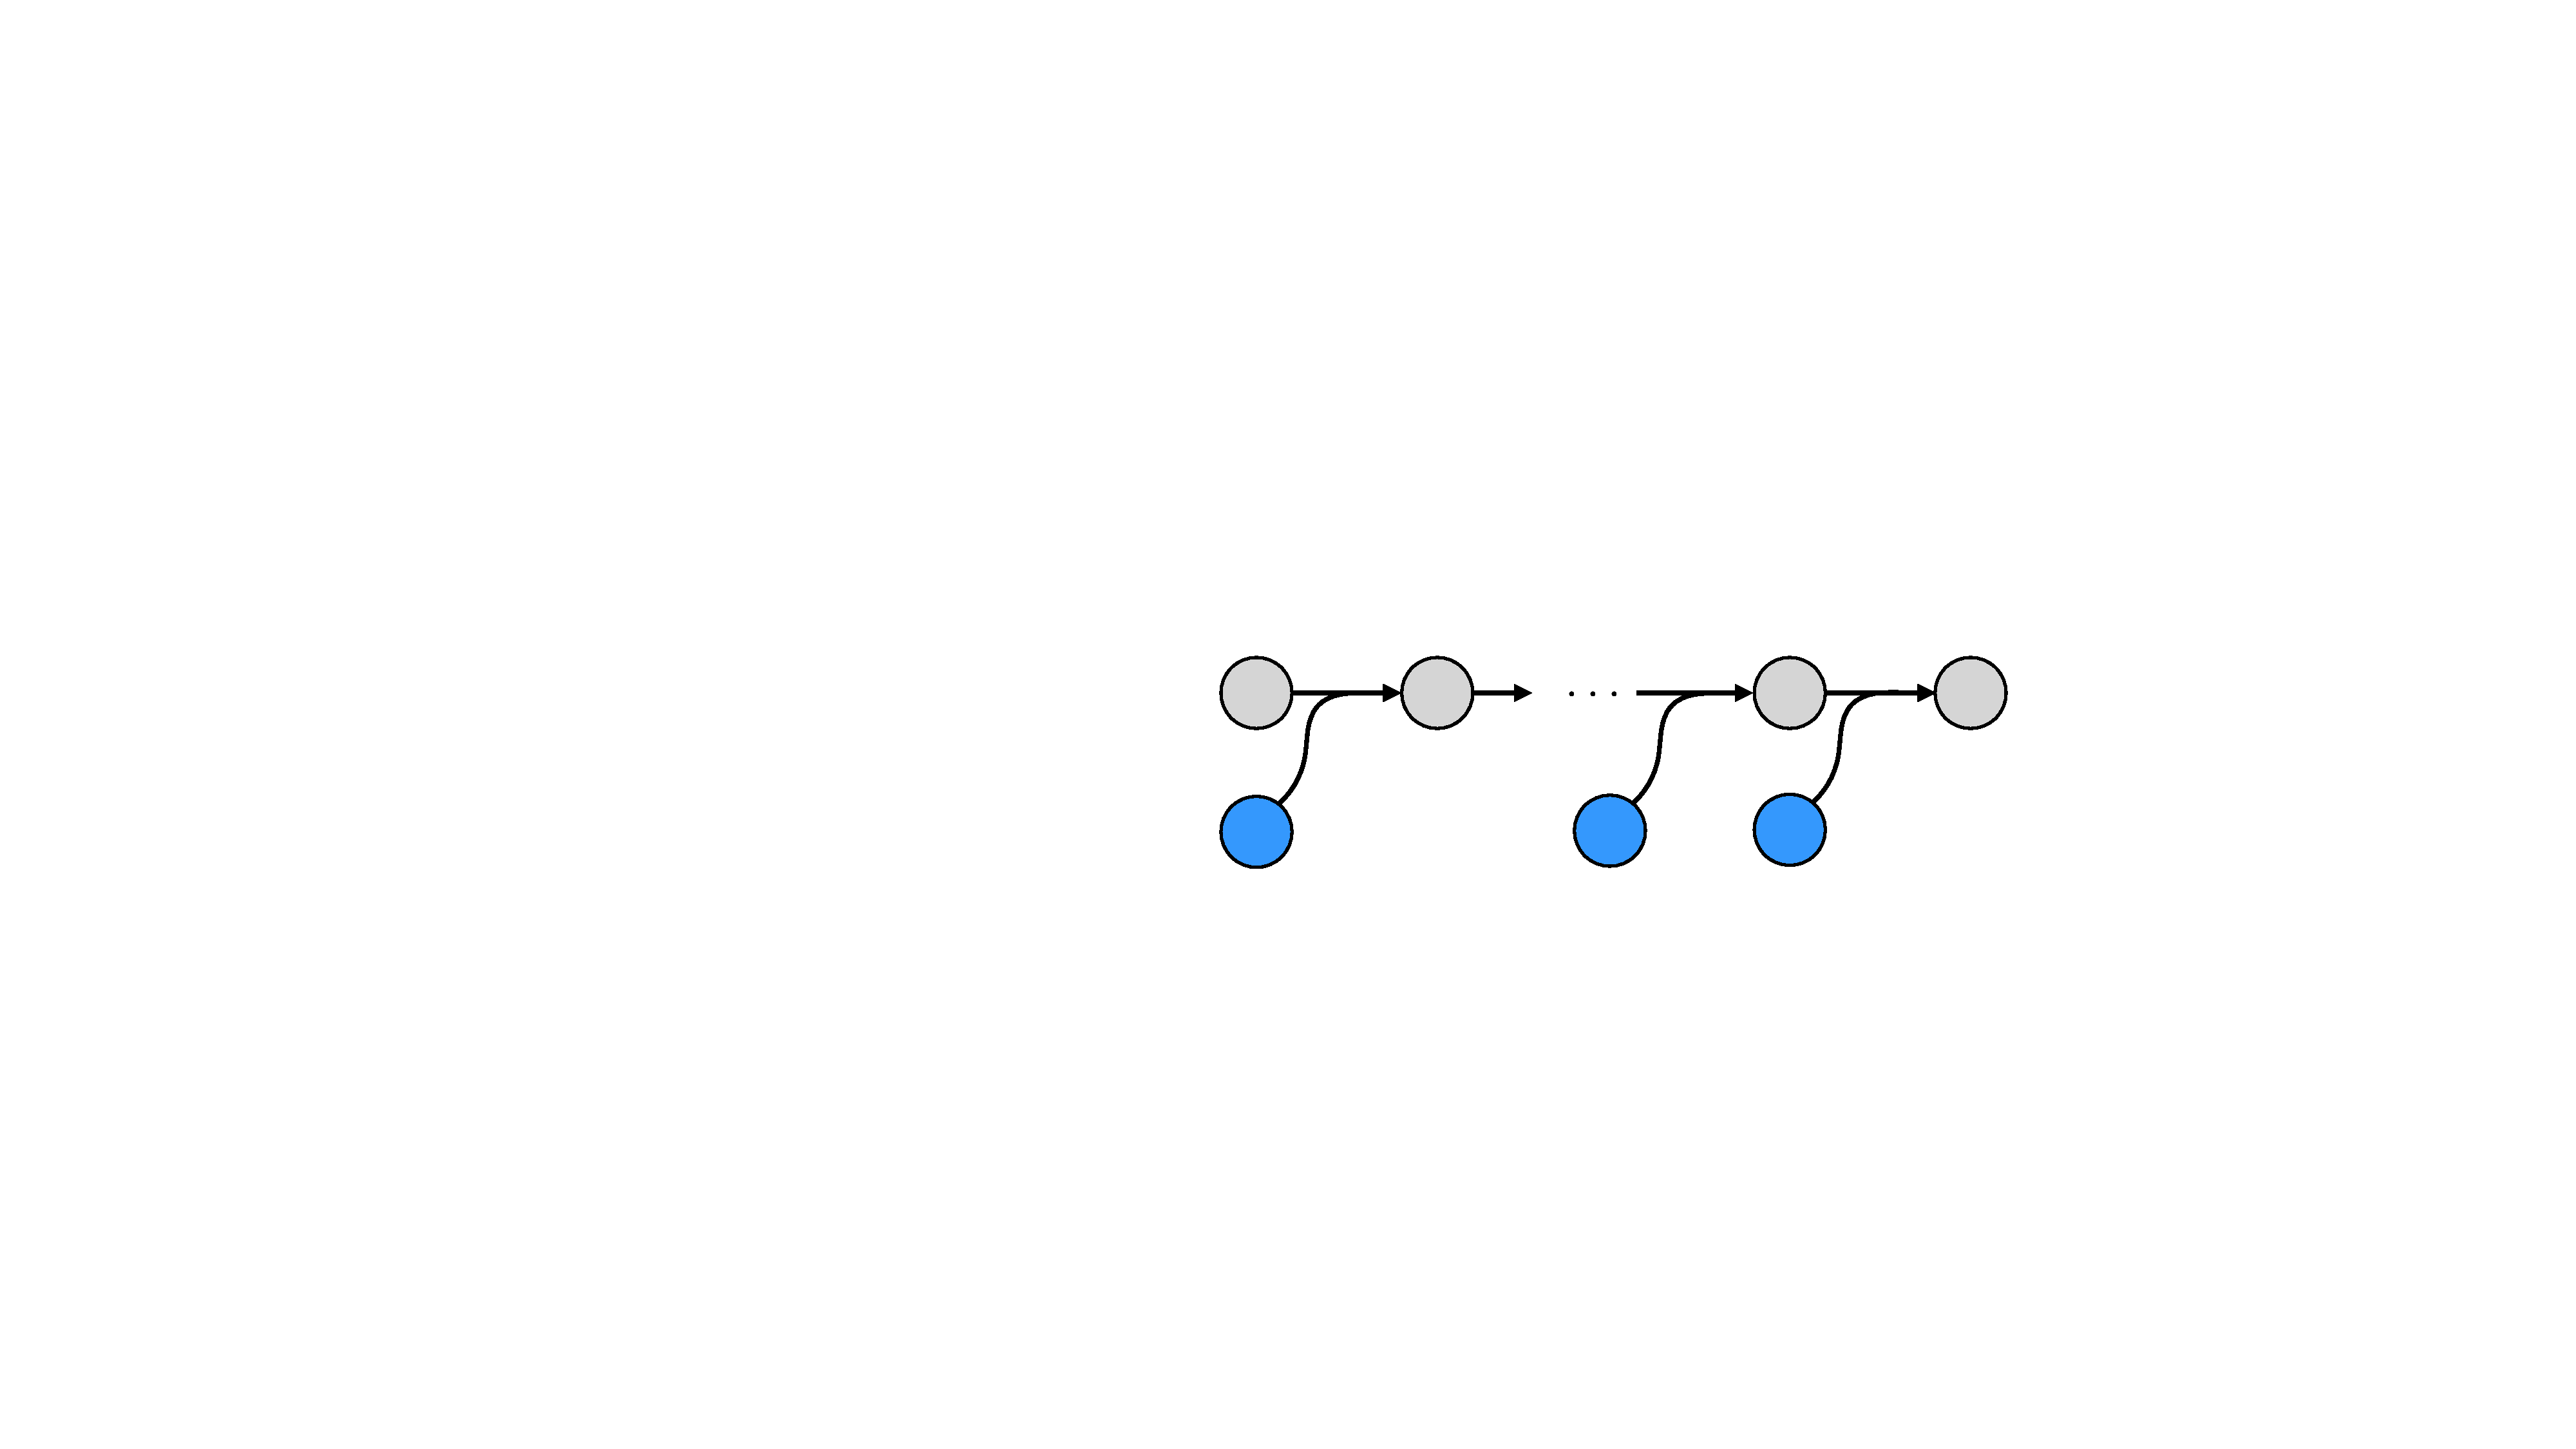
\includegraphics[width=0.45\linewidth]{./figures/backpropagation/cgraph_tree.pdf}
}
The parameters, along with the input training data, are the leaves of the computation graph.
}[2.4cm]

Our goal is to update all the values highlighted in blue: $\theta_1$, $\theta_2$, and so forth. To do so we need to compute the gradients $\frac{\partial J}{\partial \theta_1}$, $\frac{\partial J}{\partial \theta_2}$, etc. Each of these gradients can be calculated via the chain rule. Here is the chain rule written out for the gradients for $\theta_1$ and $\theta_2$:
\begin{align}
    \frac{\partial J}{\partial \theta_1} &= \highlight[shared_term_color]{\frac{\partial J}{\partial \mathbf{x}_L}\frac{\partial \mathbf{x}_L}{\partial \mathbf{x}_{L-1}} \cdots \frac{\partial \mathbf{x}_3}{\partial \mathbf{x}_2}} \frac{\partial \mathbf{x}_2}{\mathbf{x}_1}\frac{\partial \mathbf{x}_1}{\partial \mathbf{\theta}_1}\\
    \frac{\partial J}{\partial \theta_2} &=  \highlight[shared_term_color]{\frac{\partial J}{\partial \mathbf{x}_{L}}\frac{\partial \mathbf{x}_L}{\partial \mathbf{x}_{L-1}} \cdots \frac{\partial \mathbf{x}_3}{\partial \mathbf{x}_2}} \frac{\partial \mathbf{x}_2}{\partial \theta_2}
\end{align}
Rather than evaluating both equations separately, we notice that all the terms in each gray box are shared. We only need to evaluate this product once, and then can use it to compute both $\frac{\partial J}{\partial \theta_1}$ and $\frac{\partial J}{\partial \theta_2}$. Now notice that this pattern of reuse can be applied in the same way for $\theta_3$, $\theta_4$, and so on. This is the whole trick of backpropagation: rather than computing each layer's gradients independently, observe that they share many of the same terms, so we might as well calculate each shared term once and reuse them. \marginnote{This strategy, in general, is called {\bf dynamic programming}.}[-0.6cm]

%\section{\texttt{Backward} for a generic layer}
\section{Backward for a Generic Layer}
To come up with a general algorithm for reusing all the shared computation, we will first look at one generic layer in isolation, and see what we need in order to update its parameters (\fig{\ref{fig:backpropagation:generic_layer_g_L}}).
\begin{figure}[h]
\centerline{
\begin{tikzpicture}%[>=spaced latex]
%
\def\layerwidth{1.8}
%
\draw [thick] [comp_graph_edge] (\layerwidth*0.6,-0.35) -- (\layerwidth,-0.35);
\draw [thick] (\layerwidth*0.6,-0.75) -- (\layerwidth*0.6,-0.35);
\draw [thick] [comp_graph_edge] (\layerwidth*0.5,0) -- (\layerwidth,0);
\draw (\layerwidth*1.5,0) node [fill=comp_graph_node_bcolor,draw, inner sep=2mm, minimum height=1.3cm] {$f(\xin, \theta)$};
\draw [thick] [comp_graph_edge] (\layerwidth*2,0) -- (\layerwidth*2.4,0);
%
\draw (\layerwidth*0.6,-0.95) node [fill=comp_graph_param_bcolor] {$\theta$};
\draw (\layerwidth*0.4,0) node [fill=comp_graph_data_bcolor] {$\xin$};
\draw (\layerwidth*2.65,0) node [fill=comp_graph_data_bcolor] {$\xout$};
\draw (\layerwidth*3,0) node {$\cdots$};
\draw [thick] [comp_graph_edge] (\layerwidth*3.2,0) -- (\layerwidth*3.6,0);
\draw (\layerwidth*3.8,0) node {$J$};
\draw [thick] [comp_graph_edge] (-0.2*\layerwidth,0) -- (0.2*\layerwidth,0);
\draw (-0.4*\layerwidth,0) node {$\cdots$};
%
\draw (2.8,-1.4) node {$\underbrace{\quad\quad\quad\quad\quad\quad\quad\quad\quad\quad\quad\quad\quad}$};
\draw (2.8,-1.9) node [scale=1.2] {$\localgrad$};
\draw (5.8,-1.8) node {$\underbrace{\quad\quad\quad\quad\quad\quad\quad}$};
\draw (5.8,-2.3) node [scale=1.2] {$\costgradout$};
\draw (3.8,-2.6) node {$\underbrace{\quad\quad\quad\quad\quad\quad\quad\quad\quad\quad\quad\quad\quad\quad\quad\quad\quad\quad\quad}$};
\draw (3.8,-3.1) node [scale=1.2] {$\costgradin$};
%
\end{tikzpicture}
}
\caption{A generic layer in the computation graph. The braces represent the part of the computation graph we need to consider in order to evaluate $\costgradout$, $\localgrad$, and $\costgradin$.}
\label{fig:backpropagation:generic_layer_g_L}
\end{figure}

% Here we have introduced two new shorthands, $\localgrad$ and $\costgrad$ -- these represent arrays of partial derivatives, defined below, and they are the key arrays we need to keep track of to do backprop. They are defined as:
% %To update $\theta$ for this layer, we just need to know $\frac{\partial J}{\partial \theta}$
% %This strategy involves two key matrices: 1) the vector of derivatives of the cost $J$ w.r.t to each layer's inputs, and 2) the matrix of derivatives of the outputs of each layer with respect to its inputs. We define shorthand for these below:
% \marginnote{All these arrays represent the gradient \textit{at a single operating point} --  that of the current value of the data and parameters.}[1cm]
% \begin{align}
%     \costgrad &\triangleq \frac{\partial J}{\partial [\xin, \xout, \theta]} &&\quad\quad \triangleleft \quad \text{grad of cost}\\
%      &\quad\quad \costgradxin \triangleq \frac{\partial J}{\partial \xin} &&\quad\quad \triangleleft \quad \text{... w.r.t. layer inputs} \quad [1 \times |\xin|]\\
%      &\quad\quad \costgradxout \triangleq \frac{\partial J}{\partial \xout} &&\quad\quad \triangleleft \quad \text{... w.r.t. layer outputs} \quad [1 \times |\xout|]\\
%      &\quad\quad \costgradtheta \triangleq \frac{\partial J}{\partial \theta} &&\quad\quad \triangleleft \quad \text{... w.r.t. layer params} \quad [1 \times |\theta|]\\
%     \localgrad &\triangleq \frac{\partial \xout}{\partial [\xin, \theta]} &&\quad\quad \triangleleft \quad \text{grad of layer}\\
%     &\quad\quad \localgradx \triangleq \frac{\partial \xout}{\partial \xin} &&\quad\quad \triangleleft \quad \text{... w.r.t. layer input data} \quad [|\xout| \times |\xin|]\\
%     &\quad\quad \localgradtheta \triangleq \frac{\partial \xout}{\partial \theta} &&\quad\quad \triangleleft \quad \text{... w.r.t. layer params} \quad [|\xout| \times |\theta|]
%     %\mathbf{F}_l &\triangleq \frac{\partial \mathbf{x}_{l}}{\partial \mathbf{x}_{l-1}} = \frac{\partial f_l(\mathbf{x}_{l-1})}{\partial \mathbf{x}_{l-1}} &\quad\quad \triangleleft \quad [N \times M]
% \end{align}

% Computing $\localgrad$ is an entirely local process: for each layer, we just need to know the functional form of its derivative, $f^{\prime}$, which we then evaluate at the operating point $[\xin, \theta]$ to obtain $\localgrad = f^{\prime}(\xin,\theta)$.

% Computing $\costgrad$ is a bit trickier; it requires evaluating the chain rule, and depends on all the subsequent layers of processing, that come between the current layer and $J$. However, this can be computed iteratively: once we know $\costgrad_l$, for some layer $l$, computing $\costgrad_{l-1}$ is just one more matrix multiply! This can be summarized with the following recurrence relation:
% \begin{align}
%     \costgrad_{\texttt{in}} &= \costgrad_{\texttt{out}}\localgrad^{\mathbf{x}} &&\quad\quad \triangleleft \quad \text{``backpropagation of errors"} \label{eqn:backpropagation:backward}
% \end{align}
% This recurrence is essence of backprop: it sends ``error signals" (gradients) backwards through the network, starting at the last layer and iteratively applying Equation \ref{eqn:backpropagation:backward} to
% compute $\costgrad$ for each previous layer.
% \marginnote{Deep learning libraries like Pytorch have a \texttt{.grad} field associated with each variable (data, activations, parameters). This field reprsents $\frac{\partial J}{\partial v}$ for each variable $v$.}[-0.4cm]

% To do gradient-based learning, we need to compute the gradient of the cost w.r.t. the parameters, i.e. $\costgradtheta$. This gives us the parameter \texttt{update} step in gradient descent: 
% \begin{align}
%     \theta^{i+1} &\leftarrow \theta^{i} - \eta (\costgradtheta)^T &&\quad\quad \triangleleft \quad \texttt{update} \label{eqn:backpropagation:djdtheta}
% \end{align}
% \marginnote{The transpose is because, by convention $\theta$ is a column vector while $\costgradtheta = \frac{\partial J}{\partial \theta}$ is a row vector; see Appendix.}[-0.4cm]

% %These arrays give a simple formula for computing the gradient we need -- $\frac{\partial J}{\partial \theta}$ -- in order to \texttt{update} $\theta$ to minimize the cost:
% %\begin{align}
% %    \frac{\partial J}{\partial \theta_l} = \costgrad_l\localgrad^{\theta}_l \quad\quad \triangleleft \quad [1 \times |\xout|]\cdot[|\xout| \times |\theta|] \rightarrow [1 \times \theta]] \label{eqn:backpropagation:param_update}
% %\end{align}

% %The remaining question is just: how do we get $\costgrad_l$ and $\localgrad^{\theta}_l$ for layer $l$? 

% Now, observe that if we already knew $\costgradxout$, then computing $\costgradtheta$ would be easy, it would just be the following matrix product:
% \begin{align}
%     \costgradtheta = \frac{\partial J}{\partial \theta} = \frac{\partial J}{\partial \xout} \frac{\partial \xout}{\partial \theta} = \costgradxout \localgradtheta
% \end{align}

Here we have introduced two new shorthands, $\localgrad$ and $\costgrad$; these represent arrays of partial derivatives, defined below, and they are the key arrays we need to keep track of to do backprop. They are defined as:
%To update $\theta$ for this layer, we just need to know $\frac{\partial J}{\partial \theta}$
%This strategy involves two key matrices: 1) the vector of derivatives of the cost $J$ w.r.t to each layer's inputs, and 2) the matrix of derivatives of the outputs of each layer with respect to its inputs. We define shorthand for these below:
\marginnote{All these arrays represent the gradient \textit{at a single operating point}, namely that of the current value of the data and parameters.}[0.9cm]
\begin{align}
    %\costgrad &\triangleq \frac{\partial J}{\partial [\xin, \xout]} &&\quad\quad \triangleleft \quad \text{grad of cost}\\
    % &\quad\quad \costgradin \triangleq \frac{\partial J}{\partial \xin} &&\quad\quad \triangleleft \quad \text{... w.r.t. layer input data} \quad [1 \times |\xin|]\\
    % &\quad\quad \costgradout \triangleq \frac{\partial J}{\partial \xout} &&\quad\quad \triangleleft \quad \text{... w.r.t. layer outputs} \quad [1 \times |\xout|]\\
    \costgradl &\triangleq \frac{\partial J}{\partial \mathbf{x}_l} &&\quad\quad \triangleleft \quad \text{grad of cost with respect to } \mathbf{x}_l \quad [1 \times |\mathbf{x}_l|]\\
    \localgrad &\triangleq \frac{\partial \xout}{\partial [\xin, \theta]} &&\quad\quad \triangleleft \quad \text{grad of layer}\\
    &\quad\quad \localgrad^{\mathbf{x}} \triangleq \frac{\partial \xout}{\partial \xin} &&\quad\quad \triangleleft \quad \text{\quad with respect to layer input data} \quad [|\xout| \times |\xin|]\\
    &\quad\quad \localgrad^{\theta} \triangleq \frac{\partial \xout}{\partial \theta} &&\quad\quad \triangleleft \quad \text{\quad with respect to layer params} \quad [|\xout| \times |\theta|]
    %\mathbf{F}_l &\triangleq \frac{\partial \mathbf{x}_{l}}{\partial \mathbf{x}_{l-1}} = \frac{\partial f_l(\mathbf{x}_{l-1})}{\partial \mathbf{x}_{l-1}} &\quad\quad \triangleleft \quad [N \times M]
\end{align}

These arrays give a simple formula for computing the gradient we need, that is, $\frac{\partial J}{\partial \theta}$, in order to \texttt{update} $\theta$ to minimize the cost:
%\begin{align}
%    \frac{\partial J}{\partial \theta_l} = \costgrad_l\localgrad^{\theta}_l \quad\quad \triangleleft \quad [1 \times |\xout|]\cdot[|\xout| \times |\theta|] \rightarrow [1 \times \theta]] \label{eqn:backpropagation:param_update}
%\end{align}
\begin{align}
    \frac{\partial J}{\partial \theta} &= \underbrace{\frac{\partial J}{\partial \xout}}_{\costgradout} \underbrace{\frac{\partial \xout}{\partial \theta}}_{\localgradtheta} = \costgradout\localgradtheta\\
    \theta^{i+1} &\leftarrow \theta^{i} - \eta \Big(\frac{\partial J}{\partial \theta}\Big)^\transpose &&\quad\quad \triangleleft \quad \texttt{update} \label{eqn:backpropagation:djdtheta}
\end{align}
\marginnote{The transpose is because, by convention, $\theta$ is a column vector while $\frac{\partial J}{\partial \theta}$ is a row vector; see the Notation section prior to chapter 1.}[-0.5cm]

The remaining question is clear: how do we get $\costgrad_l$ and $\localgrad^{\theta}_l$ for each layer $l$? 

Computing $\localgrad$ is an entirely local process: for each layer, we just need to know the functional form of its derivative, $f^{\prime}$, which we then evaluate at the operating point $[\xin, \theta]$ to obtain $\localgrad = f^{\prime}(\xin,\theta)$.

Computing $\costgrad$ is a bit trickier; it requires evaluating the chain rule, and depends on all the layers between $\xout$ and $J$. However, this can be computed iteratively: once we know $\costgrad_l$, computing $\costgrad_{l-1}$ is just one more matrix multiply! This can be summarized with the following recurrence relation:
\begin{align}
    \costgrad_{\texttt{in}} &= \costgrad_{\texttt{out}}\localgrad^{\mathbf{x}} &&\quad\quad \triangleleft \quad \text{backpropagation of errors}
    \label{eqn:backpropagation:backward}
\end{align}
This recurrence is essence of backprop: it sends error signals (gradients) backward through the network, starting at the last layer and iteratively applying \eqn{\ref{eqn:backpropagation:backward}} to
compute $\costgrad$ for each previous layer.
\marginnote{Deep learning libraries like Pytorch have a \texttt{.grad} field associated with each variable (data, activations, parameters). This field represents $\frac{\partial J}{\partial v}$ for each variable $v$.}[-0.8cm]


We are finally ready to define the full \texttt{backward} function promised at the beginning of this chapter! It consists of the following operation, shown in \fig{\ref{fig:backpropagation:mod_block_backward}}, which has three inputs ($\xin, \theta, \costgrad_{\texttt{out}}$) and two outputs ($\costgrad_{\texttt{in}}$ and $\frac{\partial J}{\partial \theta}$).
\begin{figure}[h]
\centerline{
\begin{tikzpicture}%[>=spaced latex]
%
\def\layerwidth{1.8}
%
\draw [thick] [comp_graph_edge] (0.4,0.6) -- (\layerwidth*0.6,0.6);
\draw [thick] [comp_graph_edge] (\layerwidth*0.6,0) -- (0.4,0);
\draw [thick] [comp_graph_edge] (0.5,-0.6) -- (0.5,-0.95);
\draw [thick] (\layerwidth*0.6,-0.6) -- (0.5,-0.6);
\draw (\layerwidth*1.5,0) node [fill=comp_graph_node_bcolor,draw, inner sep=2mm, minimum height=1.8cm, minimum width=3.0cm] {};
\draw (\layerwidth*1.5,1.2) node {\texttt{backward}};
\draw (\layerwidth*1.5,0.6) node  {$\localgrad = f^{\prime}(\xin,\theta)$};
\draw (\layerwidth*1.5,0) node  {$\costgrad_{\texttt{in}} = \costgrad_{\texttt{out}}\localgrad^{\mathbf{x}}$};
\draw (\layerwidth*1.5,-0.6) node  {$\frac{\partial J}{\partial \theta} = \costgrad_{\texttt{out}}\localgrad^{\theta}$};
\draw [thick] [comp_graph_edge] (\layerwidth*2.8,0) -- (\layerwidth*2.4,0);
%
\draw (0.5,-1.3) node [fill=comp_graph_param_grad_bcolor] {$\frac{\partial J}{\partial \theta}$};
\draw (-0.2,0.6) node [fill=comp_graph_data_bcolor] {$\xin, \theta$};
\draw (0,0) node [fill=comp_graph_data_bcolor] {$\costgrad_{\texttt{in}}$};
\draw (\layerwidth*3,0) node [fill=comp_graph_data_bcolor] {$\costgrad_{\texttt{out}}$};
%
\end{tikzpicture}
}
\caption{\texttt{backward} for a generic layer. We use the color \raisebox{1mm}{\colorbox{comp_graph_param_grad_bcolor}{\makebox(0,0){}}} to indicate parameter gradients.}
\label{fig:backpropagation:mod_block_backward}
\end{figure}

% For any $\frac{\partial J}{\partial \theta_l}$, we have:
% \begin{align}
%     \frac{\partial J}{\partial \theta_l} = \frac{\partial J}{\partial \mathbf{x}_l}\frac{\partial \mathbf{x}_l}{\partial \theta_l}
% \end{align}
% This says that all the parameter updates can be computed with just one further matrix multiply once we know $\frac{\partial J}{\partial \mathbf{x}_l}$ for all $l$. Now, the trick is to work backwards to compute all the $\frac{\partial J}{\partial \mathbf{x}_l}$, because:
% \begin{align}
%     \frac{\partial J}{\partial \mathbf{x}_l} = \frac{\partial J}{\partial \mathbf{x}_{l+1}}\frac{\partial \mathbf{x}_{l+1}}{\partial \mathbf{x}_l}
% \end{align}
% So, once we know $\frac{\partial J}{\partial \mathbf{x}_{l+1}}$ we can compute $\frac{\partial J}{\partial \mathbf{x}_{l}}$ with just one additional matrix multiply.

%The value of the blue terms is $\frac{\partial j}{\partial \mathbf{x}_2}$. Once we have calculated this value, we can 

%Indeed, once we've computed $\frac{\partial \mathbf{x}_{L}}{\partial \mathbf{x}_{l}}$, we can compute $\frac{\partial \mathbf{x}_{L}}{\partial \mathbf{x}_{l-1}}$ with just one more multiply:
%\begin{align}
%    \frac{\partial \mathbf{x}_{L}}{\partial \mathbf{x}_{l-1}} = \frac{\partial \mathbf{x}_{L}}{\partial \mathbf{x}_{l}} \frac{\partial \mathbf{x}_{l}}{\partial \mathbf{x}_{l-1}}
%\end{align}

%\section{Backprop through chains}


% \begin{align}
%     \xout &= f(\xin,\theta) &&\quad\quad \triangleleft \quad \texttt{forward}\\
%     \costgrad_{\texttt{in}} &= \costgrad_{\texttt{out}}\localgrad^{\mathbf{x}} &&\quad\quad \triangleleft \quad \texttt{backward}
% \end{align}

% And then update parameters:
% \begin{align}
%     \frac{\partial J}{\partial \theta} &= \costgrad_{\texttt{out}}\localgrad^{\theta} &&\quad\quad \triangleleft \quad \texttt{update}
% \end{align}


\section{The Full Algorithm: Forward, Then Backward}
We are ready now to define the full backprop algorithm. In the last section we saw that we can easily compute the gradient update for $\theta_l$ once we have computed $\localgrad_l$ and $\costgrad_l$.\marginnote{The $\costgrad_l$ and $\localgrad_l$ are the $\costgrad$ and $\localgrad$ arrays for layer $l$.}[-0.0cm]

So, we just need to order our operations so that when we get to updating layer $l$ we have these two arrays ready. The way to do it is to first compute a \textbf{forward pass} through the entire network, which means starting with input data $\mathbf{x}_0$ and evaluating layer by layer to produce the sequence $\mathbf{x}_0, \mathbf{x}_1, \ldots, \mathbf{x}_L$. \Fig{\ref{fig:backpropagation:forward_pass}} shows what the forward pass looks like.
\begin{figure}[h]
    \centerline{
    \def\layerwidth{1.3}
    \begin{tikzpicture}[
    cblock/.style={
    draw,
    fill=comp_graph_node_bcolor,
    rectangle, 
    inner sep=1.5mm,
    minimum width=\layerwidth*0.9 cm,
    minimum height=\layerwidth*0.75*0.9 cm}]
    %
    %
    % draw f nodes
    \def\fnames {{"$f_0$","$f_1$","$f_2$","$f_{L-1}$","$f_L$"}}
    \foreach \x in {1,2,3,4} {
        \pgfmathparse{\fnames[\x]};
        \draw ($(\layerwidth*2*\x-\layerwidth+\layerwidth*0.5,0)$) node [cblock] {\pgfmathresult};
    }
    % draw data arrows
    \draw [thick] [comp_graph_edge_forward] (\layerwidth*0.5,0) -- (\layerwidth,0);
    \foreach \x in {1,2,3,4} {
        % data arrow
        \draw [thick] [comp_graph_edge_forward] (\layerwidth*2*\x,0) -- (\layerwidth*2*\x+\layerwidth,0);
    }
    %\draw [thick] [comp_graph_edge_forward] (\layerwidth*10,0) -- (\layerwidth*10.25,0);
    %
    % draw param arrows
    \foreach \x in {0,1,2,3} {
        \draw [thick] [comp_graph_edge_forward] (\layerwidth*2*\x+\layerwidth*0.6,-0.35) -- (\layerwidth*2*\x+\layerwidth,-0.35);
    }
    %
    % draw data and params
    \def\datanames {{"$\mathbf{x}_0$","$\mathbf{x}_1$","$\cdots$","$\mathbf{x}_{L-1}$","$\mathbf{x}_L$"}}
    \def\paramnames {{"$\theta_1$","$\theta_2$","$\theta_{L-1}$","$\theta_{L}$"}}
    \foreach \x in {0,1,2,3,4} {
        \pgfmathparse{\datanames[\x]};
        \draw ($(\layerwidth*2*\x+\layerwidth*0.5,0)$) node [fill=white] {\pgfmathresult};
        %
    };
    \foreach \x in {0,1,2,3} {
        \pgfmathparse{\paramnames[\x]};
        \draw ($(\layerwidth*2*\x+\layerwidth*0.5,-0.4)$) node [fill=white] {\pgfmathresult};
    };
    %
    % loss node
    \draw (\layerwidth*9.5,0) node [cblock, fill=comp_graph_loss_node_bcolor] {$\mathcal{L}$};
    %\draw (\layerwidth*10.4,0) node [fill=comp_graph_data_bcolor] {$J$};
    %
    %\draw (\layerwidth*5.5,1.0) node {\textbf{Forward pass}};
    %
    \end{tikzpicture}
    }
    \caption{Forward pass.}
    \label{fig:backpropagation:forward_pass}
\end{figure}
\marginnote{We use the color \raisebox{1mm}{\colorbox{forwardpropcolor}{\makebox(0,0){}}} for data/activations being passed forward through the network.}[2.0cm]

%We need this sequence because, in general, $\localgrad$ for a layer will be a function of $\xin$ and $\theta$ for that layer -- so we need the full sequence of inputs and outputs to each layer to get compute the full sequence $\localgrad_1, \localgrad_2, \ldots$. 

Next, we compute a \textbf{backward pass}, iteratively evaluating the $\costgrad$'s and obtaining the sequence $\costgrad_L, \costgrad_{L-1}, \ldots$, as well as the parameter gradients for each layer (\fig{\ref{fig:backpropagation:backward_pass}}). %Remember that to compute $\costgrad$ for a layer, we need $\localgrad$ for that layer, so on the
\begin{figure}[h]
    \centerline{
    \def\layerwidth{1.3}
    \begin{tikzpicture}[
    cblock/.style={
    draw,
    fill=comp_graph_node_bcolor,
    rectangle, 
    inner sep=1.5mm,
    minimum width=\layerwidth*0.9 cm,
    minimum height=\layerwidth*0.75*0.9 cm}]
    %
    %
    % draw f nodes
    \def\fnames {{"$f^{\prime}_0$","$f^{\prime}_1$","$f^{\prime}_2$","$f^{\prime}_{L-1}$","$f^{\prime}_L$"}}
    \foreach \x in {1,2,3,4} {
        \pgfmathparse{\fnames[\x]};
        \draw ($(\layerwidth*2*\x-\layerwidth+\layerwidth*0.5,0)$) node [cblock] {\pgfmathresult};
    }
    % draw data arrows
    \draw [thick] [comp_graph_edge_backward] (\layerwidth,0) -- (\layerwidth*0.7,0);
    \foreach \x in {1,2,3,4} {
        % data arrow
        \draw [thick] [comp_graph_edge_backward] (\layerwidth*2*\x+\layerwidth,0) -- (\layerwidth*2*\x,0);
    }
    \draw [thick] [comp_graph_edge_backward] (\layerwidth*10.25,0) -- (\layerwidth*10,0);
    %
    % draw data and params
    \def\datanames {{"$\costgrad_0$","$\costgrad_1$","$\cdots$","$\costgrad_{L-1}$","$\costgrad_L$"}}
    \def\paramnames {{"$\frac{\partial J}{\partial \theta_1}$","$\frac{\partial J}{\partial \theta_2}$","$\frac{\partial J}{\partial \theta_{L-1}}$","$\frac{\partial J}{\partial \theta_{L}}$"}}
    \foreach \x in {0,1,2,3,4} {
        \pgfmathparse{\datanames[\x]};
        \draw ($(\layerwidth*2*\x+\layerwidth*0.5,0)$) node [fill=comp_graph_data_bcolor] {\pgfmathresult};
        %
    };
    \foreach \x in {0,1,2,3} {
        \pgfmathparse{\paramnames[\x]};
        \draw ($(\layerwidth*2*\x+\layerwidth*0.5,-0.5)$) node [fill=white] {\pgfmathresult};
    };
    % draw param arrows
    \foreach \x in {0,1,2,3} {
        \draw [thick] [comp_graph_edge_backward] (\layerwidth*2*\x+\layerwidth,-0.35) -- (\layerwidth*2*\x+\layerwidth*0.8,-0.35);
    }
    %
    % loss node
    \draw (\layerwidth*9.5,0) node [cblock, fill=comp_graph_loss_node_bcolor] {$\mathcal{L}^{\prime}$};
    \draw (\layerwidth*10.4,0) node [fill=comp_graph_data_bcolor] {$1$};
    %
    %\draw (\layerwidth*5.5,1.0) node {\textbf{Backward pass}};
    %
    \end{tikzpicture}
    }
    \caption{Backward pass.}
    \label{fig:backpropagation:backward_pass}
\end{figure}
\marginnote{We use the color \raisebox{1mm}{\colorbox{backwardpropcolor}{\makebox(0,0){}}} for data/activation gradients being passed backward through the network.}[2cm]

%Finally, we have all the arrays necessary to compute the gradients $\frac{\partial J}{\partial \theta_l}$ for all $l$ and update all the parameters in the computation graph. 
%Finally, we update our parameters based on the gradients $\frac{\partial J}{\partial \theta_l}$, and repeat. 
The full algorithm is summarized in \algref{\ref{alg:backpropagation:backprop_for_chains}}. %A graphical depiction is given in Figure \ref{fig:backpropagation:backprop_alg_diagram}.

\begin{algorithm}[h]
\SetAlgoVlined
\DontPrintSemicolon
%\marginnote{{\bf Algorithm \ref{alg:backpropagation:backprop_for_chains}}: A simple version of the backpropagation algorithm. This will work for the computation graphs we have seen so far, which consist of a series of layers, $f_1 \circ \ldots \circ f_L$, with no merging or branching (see \sect{\ref{sec:backpropagation:branch_and_merge}} for how to handle more complicated graphs with merge and branch operations).}
\caption{{\bf Algorithm \ref{alg:backpropagation:backprop_for_chains}}: Backpropagation (for chain computation graphs). A simple version of the backpropagation algorithm. This will work for the computation graphs we have seen so far, which consist of a series of layers, $f_1 \circ \ldots \circ f_L$, with no merging or branching (see \sect{\ref{sec:backpropagation:branch_and_merge}} for how to handle more complicated graphs with merge and branch operations).}
\fakealgorithmcaption{}
\label{alg:backpropagation:backprop_for_chains}
{\bf Input:} parameter vector $\theta = \{\theta_l\}_{l=1}^L$, $f_1, \ldots, f_L$, $f^{\prime}_1, \ldots, f^{\prime}_L$, training datapoint $\{\mathbf{x}_0,\mathbf{y}\}$, Loss function $\mathcal{L}: \mathbb{R}^N \rightarrow \mathbb{R}$\;
{\bf Output:} gradient direction $\frac{\partial J}{\partial \theta} = \Big\{\frac{\partial J}{\partial \theta_l}\Big\}_{l=1}^L$ \;
\;
\textbf{Forward pass:}\;
\For{\upshape $l=1, \dots, L$} {
    $\mathbf{x}_l = f_l(\mathbf{x}_{l-1}, \theta_l)$\;
}
%$J = \mathcal{L}(\mathbf{x}_L,y)$\;
\;
\textbf{Backward pass:}\;
$\costgrad_L = \mathcal{L}^{\prime}(\mathbf{x}_L,y)$\;
\For{\upshape $l=L, \dots, 1$} {
    $\localgrad_{l} = f_l^{\prime}(\mathbf{x}_{l-1},\theta_l)$\;
    $\costgrad_{l-1} = \costgrad_{l}\localgrad^{\mathbf{x}}_{l}$\;
    $\frac{\partial J}{\partial \theta_l} = \costgrad_{l}\localgrad^{\theta}_{l}$\;
}
\end{algorithm}

\section{Backpropagation Over Data Batches}
So far, we have only examined computing the gradient of the loss for a single datapoint, $\mathbf{x}$. As you may recall from \chaps{\ref{chapter:intro_to_learning}} and \ref{chapter:gradient_descent}, the total cost function we wish to minimize will typically be the \textit{average} of the losses over \textit{all} the datapoints in a training set, $\{\mathbf{x}^{(i)}\}_{i=1}^N$. However, once we know how to compute the gradient for a single datapoint, we can easily compute the gradient for the whole dataset, due to the following identity:
\begin{align}
    \frac{\partial \frac{1}{N}\sum_{i=1}^N J_i(\theta)}{\partial \theta} = \frac{1}{N} \sum_{i=1}^N \frac{\partial J_i(\theta)}{\partial \theta}\label{eqn:backpropagation:average_of_gradients}
\end{align}
\marginnote{The gradient of a sum of terms is the sum of the gradients of each term.}[-1.0cm]
where $J_i(\theta)$ is the loss for a single datapoint $\mathbf{x}^{(i)}$. Therefore, to compute a gradient update for an algorithm like stochastic gradient descent (\sect{\ref{sec:gradient_descent:SGD}}), we apply backpropagation in batch mode, that is, we run it over each datapoint in our batch (which can be done in parallel) and then average the results.

In the remaining sections, we will still focus only on the case of backpropagation for the loss at a single datapoint. As you read on, keep in mind that doing the same for batches simply requires applying \eqn{\ref{eqn:backpropagation:average_of_gradients}}.

% The beauty of this algorithm is that each layer's job is to compute just two simple and local operations: run $\texttt{forward}$ on the forward pass, and run $\texttt{backward}$ on the backward pass. Here is the job of a generic layer: \marginnote{Notice that while the forward pass evaluates an arbitrary function, $f_l$, specific to the layer type, the backward pass is \textit{always} a vector-matrix product, regardless of the functional form of $f_l$.}[-0.2cm]
% \begin{figure}[h]
% \centering
% \begin{tikzpicture}%[>=spaced latex]
% %
% \def\layerwidth{1.8}
% %
% % node
% \draw (\layerwidth*2.25,0) node [fill=comp_graph_node_bcolor,draw, inner sep=2mm, minimum height=1.3cm, minimum width=3.5cm] {};
% \draw (\layerwidth*2.25,0.25) node {$\mathbf{x}_l = f_l(\mathbf{x}_{l-1},\theta)$};
% \draw (\layerwidth*2.25,-0.25) node {$\costgrad_{l-1} = \costgrad_l\localgrad^{\mathbf{x}}_l$};
% %
% % forward pass
% % edge in
% \draw [thick] [comp_graph_edge_forward] (\layerwidth*0.75,0.25) -- (\layerwidth*1.25,0.25);
% % edge out
% \draw [thick] [comp_graph_edge_forward] (\layerwidth*3.25,0.25) -- (\layerwidth*3.65,0.25);
% % inputs
% \draw (\layerwidth*0.45,0.25) node [fill=comp_graph_data_bcolor] {$\mathbf{x}_{l-1}, \theta$};
% % outputs
% \draw (\layerwidth*3.8,0.25) node [fill=comp_graph_data_bcolor] {$\mathbf{x}_l$};
% %
% % backward pass
% % edge in
% \draw [thick] [comp_graph_edge_backward] (\layerwidth*1.25,-0.25) -- (\layerwidth*0.75,-0.25);
% % edge out
% \draw [thick] [comp_graph_edge_backward] (\layerwidth*3.65,-0.25) -- (\layerwidth*3.25,-0.25);
% % inputs
% \draw (\layerwidth*3.8,-0.25) node {$\costgrad_l$};
% % outputs
% \draw (\layerwidth*0.45,-0.25) node {$\costgrad_{l-1}$};
% %
% \end{tikzpicture}
% \end{figure}


%On the forward pass ($\textcolor{forwardpropcolor}{\rightarrow}$), each layer gets inputs $[\mathbf{x}_{l-1},\theta]$ and produces outputs $\mathbf{x}_l$. On the backward pass ($\textcolor{backwardpropcolor}{\leftarrow}$) each layer gets input $\costgrad_l$. and produces output $\costgrad_{l-1}$. After the complete forward and backward passes, we can update all parameters with Equation \ref{eqn:backpropagation:param_update}.


\section{Example: Backpropagation for an MLP}

%\marginnote{We need to run the forward pass before the backward pass because $\texttt{backward}$ for each layer requires as input not just $\costgrad_{\texttt{out}}$ but also $\xin$, which we only will know after running the forward pass.}[-8.0cm]

In order to fully describe backprop for any given architecture, we need $\localgrad$ for each layer in the network. One way to do this is to define the derivative $f^{\prime}$ for all atomic functions like addition, multiplication, and so on, and then expand every layer into a computation graph that involves just these atomic operations. Backprop through the expanded computation graph will then simply make use of all the atomic $f^{\prime}$s to compute the necessary $\localgrad$ matrices. However, often there are more efficient ways of writing \texttt{backward} for standard layers. In this section we will derive a compact \texttt{backward} for linear layers and relu layers — the two main layers in MLPs.

\subsection{Backpropagation for a Linear Layer}

The definition of a linear layer, in forward direction, is as follows:
\begin{align}
    \xout = \mathbf{W} \xin + \mathbf{b}
\end{align}
We have separated the parameters into $\mathbf{W}$ and $\mathbf{b}$ for clarity, but remember that we could always rewrite the following in terms of $\theta = \texttt{vec}[\mathbf{W}, \mathbf{b}]$.\marginnote{The \texttt{vec} is the vectorization operator, which takes numbers in some structured format and rearranges them into a vector.} Let $\xin$ be $N$-dimensional and $\xout$ be $M$-dimensional; then $\mathbf{W}$ is an $[M \times N]$ dimensional matrix and $\mathbf{b}$ is an $M$-dimensional vector.

Next we need the gradients of this function, with respect to its inputs and parameters, that is, $\localgrad$. Matrix algebra typically hides the details so we will instead first write out all the individual scalar gradients:
\marginnote{Here we define $\localgrad^\mathbf{W}$ and $\localgrad^\mathbf{b}$ as matrices that store the gradients of each output with respect to each weight and bias, respectively. The columns of $\localgrad^\mathbf{W}$ index over all the $MN$ weights.}[0.8cm]
\begin{align}
    \localgrad^{\mathbf{x}}[i,j] &= \frac{\partial x_{\texttt{out}}[i]}{\partial x_{\texttt{in}}[j]} = 
    \frac{\partial \sum_l \mathbf{W}[i,l] x_{\texttt{in}}[l]}{\partial x_{\texttt{in}}[j]} = \mathbf{W}[i,j] \label{lingrad1}\\
    %\quad\quad \rightarrow \boxed{\localgrad^{\mathbf{x}} = \mathbf{W}}\\% \quad \triangleleft [M \times N]\\
    %
    \localgrad^{\mathbf{W}}[i,jk] &= \frac{\partial x_{\texttt{out}}[i]}{\partial \mathbf{W}[j,k]} = \frac{\partial \sum_l \mathbf{W}[i,l] x_{\texttt{in}}[l]}{\partial \mathbf{W}[j,k]} = 
    \begin{cases}
        x_{\texttt{in}}[k], &\text{if} \quad i == j\\
        0,      & \text{otherwise}
    \end{cases} \label{lingrad2}\\
    %
    \localgrad^{\mathbf{b}}[i,j] &= \frac{\partial x_{\texttt{out}}[i]}{\partial \mathbf{b}[j]} = 
    \begin{cases}
        1, &\text{if} \quad i == j\\
        0, & \text{otherwise}
    \end{cases} \label{lingrad3}
    %\quad\quad \rightarrow \boxed{\localgrad^{\mathbf{b}} = \mathbf{I}}% \quad \triangleleft [M \times M]
\end{align}

\Eqns{\ref{lingrad1}} and (\ref{lingrad3}) imply:
\begin{align}
    \boxed{\localgrad^{\mathbf{x}} = \mathbf{W}} &\quad\quad \triangleleft \quad [M \times N]\\
    \boxed{\localgrad^{\mathbf{b}} = \mathbf{I}} &\quad\quad \triangleleft \quad [M \times M]
\end{align}
There is no such simple shorthand for $\localgrad^\mathbf{W}$, but that is no matter, as we can proceed at this point to implement \texttt{backward} for a linear layer by plugging our computed $\localgrad^\mathbf{x}$ into \eqn{\ref{eqn:backpropagation:backward}}, and $\localgrad^\mathbf{W}$ and $\localgrad^\mathbf{b}$ into \eqn{\ref{eqn:backpropagation:djdtheta}}.
%\marginnote{Note that $\frac{\partial J}{\partial \texttt{vec}(\mathbf{W})}$ is w.r.t. the vectorized list of parameters in $\mathbf{W}$, consistent with Equation \ref{lingrad2}.}
\begin{align}
    \costgrad_{\texttt{in}} &= \costgrad_{\texttt{out}}\localgrad^{\mathbf{x}} = \costgrad_{\texttt{out}}\mathbf{W} \label{eqn:backpropagation:linear_backward_costgrad}\\
    \frac{\partial J}{\partial \mathbf{W}} &=  \costgrad_{\texttt{out}}\localgrad^{\mathbf{W}}\\
    \frac{\partial J}{\partial \mathbf{b}} &= \costgrad_{\texttt{out}}\localgrad^{\mathbf{b}} = \costgrad_{\texttt{out}}
\end{align}
To get an intuition for \eqn{\ref{eqn:backpropagation:linear_backward_costgrad}}, it can help to draw the matrices being multiplied. Below, in \fig{\ref{fig:backpropagation:linear_forward_backward_matrices}}, on the left we have the forward operation of the layer (omitting biases) and on the right we have the backward operation in \eqn{\ref{eqn:backpropagation:linear_backward_costgrad}}.
\begin{figure}[h]
\centerline{
\begin{minipage}{0.33\linewidth}
\begin{tikzpicture}
\draw[step=0.25cm,draw=black,fill=forwardpropcolor] (0,0) grid (0.25,-0.75) rectangle (0,0); \node at (0.125,0.25) {$\xout$};
\draw (0.5,-0.15) node {$=$};
\draw[step=0.25cm,draw=black,fill=comp_graph_param_bcolor] (0.75,0) grid (1.75,-0.75) rectangle (0.75,0); \node at (1.25,0.25) {$\mathbf{W}$};
\draw[step=0.25cm,draw=black,fill=forwardpropcolor,shift={(0.125,0)}] (1.75,0) grid (2.0,-1.0) rectangle (1.75,0); \node at (2.0,0.25) {$\xin$};
\draw (1.0,0.75) node {\texttt{forward}};
\end{tikzpicture}
\end{minipage}
%
\begin{minipage}{0.33\linewidth}
\begin{tikzpicture}
\draw[step=0.25cm,draw=black,fill=backwardpropcolor] (0,0) grid (1.0,-0.25) rectangle (0,0); \node at (0.5,0.25) {$\costgrad_{\texttt{in}}$};
\draw (1.25,-0.15) node {$=$};
\draw[step=0.25cm,draw=black,fill=backwardpropcolor] (1.5,0) grid (2.25,-0.25) rectangle (1.5,0); \node at (1.875,0.25) {$\costgrad_{\texttt{out}}$};
\draw[step=0.25cm,draw=black,fill=comp_graph_param_bcolor,shift={(0.875,0)}] (1.5,0) grid (2.5,-0.75) rectangle (1.5,0); \node at (2.875,0.25) {$\mathbf{W}$};
\draw (1.45,0.75) node {\texttt{backward}};
\end{tikzpicture}
\end{minipage}
}
\caption{The \texttt{forward} and \texttt{backward} matrix multiples for a linear layer.}
\label{fig:backpropagation:linear_forward_backward_matrices}
\end{figure}

Unlike the other equations, at first glance $\frac{\partial J}{\partial \mathbf{W}}$ does not seem to have a simple form. A naive approach would be to first build out the large sparse matrix $\localgrad^{\mathbf{W}}$ (which is $[M \times MN]$, with zeros wherever $i \neq k$ in $\localgrad^\mathbf{W}[i,jk]$), then do the matrix multiply $\costgrad_{\texttt{out}}\localgrad^{\mathbf{W}}$. We can avoid all those multiplications by zero by observing the following simplification:
%If we adopt the convention that Jacobians $\frac{\partial \mathbf{y}}{\partial \mathbf{x}}$ are written with $\partial \mathbf{y}_i$ indexed along the rows and $\partial \mathbf{x}_j$ indexed along the columns, 
%We can collate all the indices in Equations \ref{lingrad1} and \ref{lingrad3} into simple compact forms:
% \begin{align}
%     \frac{\partial \xout}{\partial \xin} &= \mathbf{W} & \quad\quad \triangleleft \quad [M \times N]\\
%     \frac{\partial \xout}{\partial \mathbf{b}} &= \mathbf{I} & \quad\quad \triangleleft \quad [M \times M]
% \end{align}
%The same doesn't work for $\frac{\partial \xout}{\mathbf{W}}$, since we have not defined a compact notation for gradients of a vector with respect to a matrix. We will set it aside for the moment.

% Now we can compute the gradients with respect to the loss via the chain rule, using Equations \ref{update_x} and \ref{update_theta}.
% \begin{align}
%     \frac{\partial \mathcal{L}}{\partial \xin} = \frac{\partial \mathcal{L}}{\partial \xout} \frac{\partial \xout}{\partial \xin} = \frac{\partial \mathcal{L}}{\partial \xout}\mathbf{W} & \quad\quad \triangleleft [1 \times M][M \times N] \rightarrow [1 \times N]\\
%     \frac{\partial \mathcal{L}}{\partial \mathbf{b}} = \frac{\partial \mathcal{L}}{\partial \xout} \frac{\partial \xout}{\partial \mathbf{b}} = \frac{\partial \mathcal{L}}{\partial \xout} \mathbf{I} & \quad\quad \triangleleft [1 \times M][M \times M] \rightarrow [1 \times M]
% \end{align}

%We still need the gradient of the loss with respect to $\mathbf{W}$. First, we will write out the gradient with respect to each term $\mathbf{W}_{ij}$, then we will see that the update collapses to a compact form.
\begin{align}
    \frac{\partial J}{\partial \mathbf{W}[i,j]} 
        &= \frac{\partial J}{\partial \xout} \frac{\partial \xout}{\partial \mathbf{W}[i,j]} \quad\quad\quad\quad\quad\quad \triangleleft \quad[1 \times M][M \times 1] \rightarrow [1 \times 1]\\
        &= \frac{\partial J}{\partial \xout} \Big[\frac{\partial x_{\texttt{out}}[0]}{\partial \mathbf{W}[i,j]}, \ldots ,\frac{\partial x_{\texttt{out}}[M-1]}{\partial \mathbf{W}[i,j]} \Big]^\transpose \\
        &= \frac{\partial J}{\partial \xout} \Big[\ldots , 0, \ldots , \frac{\partial x_{\texttt{out}}[i]}{\partial \mathbf{W}[i,j]}, \ldots, 0, \ldots \Big]^\transpose \\
        &= \frac{\partial J}{\partial \xout} \Big[\ldots , 0, \ldots , x_{\texttt{in}}[j], \ldots, 0, \ldots \Big]^\transpose \\
        &= \frac{\partial J}{\partial x_{\texttt{out}}[i]}x_{\texttt{in}}[j] \quad\quad\quad\quad\quad\quad \triangleleft \quad[1 \times 1][1 \times 1] \rightarrow [1 \times 1]
\end{align}
\marginnote{In matrix equations, it's very useful to check that the dimensions all match up. To the right of some equations in this chapter, we denote the dimensionality of the matrices in the product, where $\xin$ is M dimensions, $\xout$ is N dimensions, and the loss $J$ is always a scalar.}[-5.0cm]
Now we can just arrange all these scalar derivatives into the matrix for $\frac{\partial J}{\partial \mathbf{W}}$, and obtain the following:
\begin{align}
    \frac{\partial J}{\partial \mathbf{W}} & = 
        \begin{bmatrix}
            \frac{\partial J}{\partial \mathbf{W}[0,0]} & \ldots & \frac{\partial J}{\partial \mathbf{W}[N-1,0]} \\
            \vdots & \ddots & \vdots \\
            \frac{\partial J}{\partial \mathbf{W}[0,M-1]} & \ldots & \frac{\partial J}{\partial \mathbf{W}[N-1,M-1]} \\
        \end{bmatrix}\\
        & = 
        \begin{bmatrix}
            \frac{\partial J}{\partial x_{\texttt{out}}[0]}x_{\texttt{in}}[0] & \ldots & \frac{\partial J}{\partial x_{\texttt{out}}[N-1]}x_{\texttt{in}}[0] \\
            \vdots & \ddots & \vdots \\
            \frac{\partial J}{\partial x_{\texttt{out}}[0]}x_{\texttt{in}}[M-1] & \ldots & \frac{\partial J}{\partial x_{\texttt{out}}[N-1]}x_{\texttt{in}}[M-1] \\
        \end{bmatrix}\\
        & = \xin \frac{\partial J}{\partial \xout}\\
        &= \xin \costgrad_{\texttt{out}}
\end{align}
\marginnote{Note, we are using the convention of zero-indexing into vectors and matrices.}[-4.0cm]
So we see that in the end this gradient has the simple form of an outer product between two vectors, $\xin$ and $\costgrad_{\texttt{out}}$ (\fig{\ref{fig:backpropagation:parameter_grad_linear_matrices}}).  %Plugging these gradients into the parameter update rule we have:
% \begin{align}
%     \mathbf{W}^{t+1} &\leftarrow \mathbf{W}^t + \eta (\xin \frac{\partial \mathcal{L}}{\partial \xout})^T\\
%     \mathbf{b}^{t+1} &\leftarrow \mathbf{b}^t + \eta (\frac{\partial \mathcal{L}}{\partial \xout})^T
% \end{align}
% where we had to transpose $\frac{\partial \mathcal{L}}{\partial \xout}$ and $\xin \frac{\partial \mathcal{L}}{\partial \xout}$ so that the indices line up (remember how the shapes got transposed, by convention, in Equations \ref{backprop:scalar_vector_deriv} and  \ref{backprop:scalar_matrix_deriv}).

\begin{figure}[h]
\centerline{
\begin{tikzpicture}
\draw[step=0.25cm,draw=black,fill=comp_graph_param_grad_bcolor] (0,0) grid (0.75,-1.0) rectangle (0,0); \node at (0.375,0.3) {$\frac{\partial J}{\partial \mathbf{W}}$};
\draw (1.0,-0.15) node {$=$};
\draw[step=0.25cm,draw=black,fill=forwardpropcolor] (1.25,0) grid (1.5,-1.0) rectangle (1.25,0); \node at (1.375,0.3) {$\xin$};
\draw[step=0.25cm,draw=black,fill=backwardpropcolor,shift={(0.125,0)}] (1.5,0) grid (2.25,-0.25) rectangle (1.5,0); \node at (2,0.3) {$\costgrad_{\texttt{out}}$};
\end{tikzpicture}
}
\caption{Matrix multiply for parameter gradient of a linear layer.}
\label{fig:backpropagation:parameter_grad_linear_matrices}
\end{figure}

We can summarize all these operations in the \texttt{forward} and \texttt{backward} diagram for linear layer in \fig{\ref{fig:backpropagation:linear_layer_backprop}}.
\begin{figure}[h]
\centerline{
\begin{tikzpicture}%[>=spaced latex]
%
\def\layerwidth{2.0}
%
\draw [thick] [comp_graph_edge_forward] (0.4,0.6) -- (\layerwidth*0.6,0.6);
\draw [thick] [comp_graph_edge_backward] (\layerwidth*0.6,0) -- (0.4,0);
\draw [thick] [comp_graph_edge_backward_params] (-0.3,-0.6) -- (-0.3,-0.95);
\draw [thick] [color=backwardpropcolor_params] (\layerwidth*0.6,-0.6) -- (-0.3,-0.6);
\draw [thick] [comp_graph_edge_backward_params] (0.5,-1.2) -- (0.5,-1.55);
\draw [thick] [color=backwardpropcolor_params] (\layerwidth*0.6,-1.2) -- (0.5,-1.2);
\draw (\layerwidth*1.5,-0.3) node [fill=comp_graph_node_bcolor,draw, inner sep=2mm, minimum height=2.6cm, minimum width=3.4cm] {};
\draw (\layerwidth*1.5,1.8) node {\textbf{linear layer}};
\draw (\layerwidth*1.5,1.4) node {\texttt{forward} and \texttt{backward}};
\draw (\layerwidth*1.5,0.6) node  {$\xout = \mathbf{W}\xin + \mathbf{b}$};
\draw (\layerwidth*1.5,0) node  {$\costgrad_{\texttt{in}} = \costgrad_{\texttt{out}}\mathbf{W}$};
\draw (\layerwidth*1.5,-0.6) node  {$\frac{\partial J}{\partial \mathbf{W}} = \xin \costgrad_{\texttt{out}}$};
\draw (\layerwidth*1.5,-1.2) node  {$\frac{\partial J}{\partial \mathbf{b}} = \costgrad_{\texttt{out}}$};
\draw [thick] [comp_graph_edge_forward] (\layerwidth*2.4,0.6) -- (\layerwidth*2.75,0.6);
\draw [thick] [comp_graph_edge_backward] (\layerwidth*2.8,-0.6) -- (\layerwidth*2.4,-0.6);
%
\draw (-0.3,-1.3) node [fill=comp_graph_param_grad_bcolor] {$\frac{\partial J}{\partial \mathbf{W}}$};
\draw (0.5,-1.9) node [fill=comp_graph_param_grad_bcolor] {$\frac{\partial J}{\partial \mathbf{b}}$};
\draw (-0.3,0.6) node [fill=comp_graph_data_bcolor] {$\xin, \mathbf{W}, \mathbf{b}$};
\draw (0,0) node [fill=comp_graph_data_bcolor] {$\costgrad_{\texttt{in}}$};
\draw (\layerwidth*3,-0.6) node [fill=comp_graph_data_bcolor] {$\costgrad_{\texttt{out}}$};
\draw (\layerwidth*3,0.6) node [fill=comp_graph_data_bcolor] {$\xout$};
%
\end{tikzpicture}
}
\caption{Linear layer \texttt{forward} and \texttt{bacward}.}
\label{fig:backpropagation:linear_layer_backprop}
\end{figure}

%This may have looked a bit complicated, but it's completely mechanical, just a lot of bookkeeping of indices. In practice we rarely derive these updates by hand; instead we use programs to automatically compute them.

Notice that all these operations are simple expressions, mainly involving matrix multiplies. \texttt{Forward} and \texttt{backward} for a linear layer are also very easy to write in code, using any library that provides matrix multiplication (\texttt{matmul}) as a primitive. \Fig{\ref{fig:backpropagation:backprop_code}} gives Python pseudocode for this layer.
\begin{figure}[h]
\begin{minipage}{1.0\linewidth}
\begin{minted}[xleftmargin=0.2\linewidth,xrightmargin=0.2\linewidth,
fontsize=\fontsize{8.5}{9},
frame=single,
framesep=2.5pt,
baselinestretch=1.05,
]{python}

class linear():
    def __init__(self, W, b, lr):
        self.W = W
        self.b = b
        self.lr = lr # learning rate
        
    def forward(self, x_in):
        self.x_in = x_in
        return matmul(W,x)+b
    
    def backward(self,J_out):
        J_in = matmul(J_out,W)
        dJdW = matmul(self.x_in,J_out)
        dJdb = J_out
        return J_in, dJdW, dJdb
    
    def update(self, dJdW, dJdb):
        self.W -= self.lr*dJdW.transpose()
        self.b -= self.lr*dJdb
\end{minted}
\end{minipage}
\caption{Pytorch-like pseudocode for a linear layer with \texttt{forward} and \texttt{backward}.}
\label{fig:backpropagation:backprop_code}
\end{figure}


\subsection{Backpropagation for a Pointwise Nonlinearity}

Pointwise nonlinearities have very simple \texttt{backward} functions. Let a (parameterless) scalar nonlinearity be $h: \mathbb{R} \rightarrow \mathbb{R}$ with derivative function $h^{\prime}: \mathbb{R} \rightarrow \mathbb{R}$. Define a  pointwise layer using $h$ as $f(\xin) = [h(x_{\texttt{in}}[0]), \ldots, h(x_{\texttt{in}}[N-1])]^\transpose$. Then we have
\begin{align}
    \localgrad^{\mathbf{x}} &= f^{\prime}(\xin) = \texttt{diag}([h^\prime(x_{\texttt{in}}[0]), \ldots, h^\prime(x_{\texttt{in}}[N-1])]^\transpose) \triangleq \mathbf{H}^\prime
\end{align}
\marginnote{The $\texttt{diag}$ is the operator that places a vector on the diagonal of a matrix, whose other entries are all zero.}[-0.4cm]
There are no parameters to update, so we just have to calculate $\costgrad_{\texttt{in}}$ in the \texttt{backward} operation, using \eqn{\ref{eqn:backpropagation:backward}}:
\begin{align}
    \costgrad_{\texttt{in}} = \costgrad_{\texttt{out}}\mathbf{H}^\prime
\end{align}

As an example, for a \texttt{relu} layer we have:
\begin{align}
    h^\prime(x) = 
        \begin{cases}
            1 &\text{if} \quad x \geq 0\\
            0 &\text{otherwise}
        \end{cases}
\end{align}
As a matrix multiply, the \texttt{backward} operation is shown in \fig{\ref{fig:backpropagation:pointwise_backward_matices}}.
\begin{figure}[h]
\centerline{
\begin{tikzpicture}
\draw[step=0.25cm,draw=black,fill=backwardpropcolor] (0.25,0) grid (1.0,-0.25) rectangle (0.25,0); \node at (0.625,0.25) {$\costgrad_{\texttt{in}}$};
\draw (1.25,-0.15) node {$=$};
\draw[step=0.25cm,draw=black,fill=backwardpropcolor] (1.5,0) grid (2.25,-0.25) rectangle (1.5,0); \node at (1.875,0.25) {$\costgrad_{\texttt{out}}$};
\draw[step=0.25cm,draw=black,fill=white,shift={(0.875,0)}] (1.5,0) grid (2.25,-0.75) rectangle (1.5,0); 
\draw[step=0.25cm,draw=black,fill=comp_graph_param_bcolor,shift={(0.875,0)}] (1.5,0) grid (1.75,-0.25) rectangle (1.5,0); 
\draw[step=0.25cm,draw=black,fill=comp_graph_param_bcolor,shift={(0.875,0)}] (1.75,-0.25) grid (2.0,-0.5) rectangle (1.75,-0.25); 
\draw[step=0.25cm,draw=black,fill=comp_graph_param_bcolor,shift={(0.875,0)}] (2.0,-0.5) grid (2.25,-0.75) rectangle (2.0,-0.5); 
\node at (2.75,0.25) {$\mathbf{H}^{\prime}$};
\node at (2.5,-0.125) {$a$};
\node at (2.75,-0.125) {$0$};
\node at (3.0,-0.125) {$0$};
\node at (2.5,-0.375) {$0$};
\node at (2.75,-0.375) {$b$};
\node at (3.0,-0.375) {$0$};
\node at (2.5,-0.625) {$0$};
\node at (2.75,-0.625) {$0$};
\node at (3.0,-0.625) {$c$};
\end{tikzpicture}
}
\caption{Matrix multiply for \texttt{backward} of a pointwise layer.}
\label{fig:backpropagation:pointwise_backward_matices}
\end{figure}

with $a = h^\prime(x_{\texttt{in}}[0])$, $b = h^\prime(x_{\texttt{in}}[1])$, and $c = h^\prime(x_{\texttt{in}}[2])$. We can simplify this equation as follows:
\begin{align}
    \costgrad_{\texttt{in}}[i] = \costgrad_{\texttt{out}}[i]h^{\prime}(\xin[i]) \quad \forall i \label{eqn:backpropagation:pointwise_costgrad}
\end{align}

The full set of operations for a pointwise layer is shown next in \fig{\ref{fig:backpropagation:pointwise_layer_backprop}}.
\begin{figure}[h]
\centerline{
\begin{tikzpicture}%[>=spaced latex]
%
\def\layerwidth{2.0}
%
\draw [thick] [comp_graph_edge_forward] (0.4,0.6) -- (\layerwidth*0.6,0.6);
\draw [thick] [comp_graph_edge_backward] (\layerwidth*0.6,0) -- (0.4,0);
\draw (\layerwidth*1.5,0.3) node [fill=comp_graph_node_bcolor,draw, inner sep=2mm, minimum height=1.6cm, minimum width=3.6cm] {};
\draw (\layerwidth*1.5,1.8) node {\textbf{pointwise layer}};
\draw (\layerwidth*1.5,1.4) node {\texttt{forward} and \texttt{backward}};
\draw (\layerwidth*1.5,0.6) node  {$\xout[i] = h(\xin[i])$};
\draw (\layerwidth*1.5,0) node  {$\costgrad_{\texttt{in}}[i] = \costgrad_{\texttt{out}}[i]h^{\prime}(\xin[i])$};
\draw [thick] [comp_graph_edge_forward] (\layerwidth*2.4,0.6) -- (\layerwidth*2.75,0.6);
\draw [thick] [comp_graph_edge_backward] (\layerwidth*2.8,0) -- (\layerwidth*2.4,0);
%
\draw (-0.1,0.6) node [fill=comp_graph_data_bcolor] {$\xin$};
\draw (0,0) node [fill=comp_graph_data_bcolor] {$\costgrad_{\texttt{in}}$};
\draw (\layerwidth*3,0.0) node [fill=comp_graph_data_bcolor] {$\costgrad_{\texttt{out}}$};
\draw (\layerwidth*3,0.6) node [fill=comp_graph_data_bcolor] {$\xout$};
%
\end{tikzpicture}
}
\caption{Pointwise layer \texttt{forward} and \texttt{backward}}
\label{fig:backpropagation:pointwise_layer_backprop}
\end{figure}


\subsection{Backpropagation for Loss Layers}
The last layer we need to define for a complete MLP is the loss layer. As a simple example, we will derive backprop for an $L_2$ loss function: $\norm{\hat{\mathbf{y}} - \mathbf{y}}^2_2$, where $\hat{\mathbf{y}}$ is the output of the network (prediction) and $\mathbf{y}$ is the ground truth.

This layer has no parameters so we only need to derive \eqn{\ref{eqn:backpropagation:backward}} for this layer:
\begin{align}
    \localgrad^{\mathbf{x}} &= \frac{\partial \norm{\hat{\mathbf{y}} - \mathbf{y}}^2_2}{\partial \hat{\mathbf{y}}} = 2(\hat{\mathbf{y}} - \mathbf{y}) \quad\quad \triangleleft \quad [1 \times |\mathbf{y}|]\\
    \costgrad_{\texttt{in}} &= \costgrad_{\texttt{out}}*2(\hat{\mathbf{y}} - \mathbf{y}) = 2(\hat{\mathbf{y}} - \mathbf{y})
\end{align}
Here we have made use of the fact that $\costgrad_{\texttt{out}} = \frac{\partial J}{\partial \xout} = \frac{\partial J}{\partial J} = 1$, since the output of the loss layer \textit{is} the cost $J$.

So, the backward signal sent by the $L_2$ loss layer is a row vector of per-dimension errors between the prediction and the target.

This completes our derivation of $\texttt{forward}$ and $\texttt{backward}$ for a $L_2$ loss layer, yielding \fig{\ref{fig:backpropagation:L2_loss_layer_backprop}}.
\begin{figure}[h]
\centerline{
\begin{tikzpicture}%[>=spaced latex]
%
\def\layerwidth{2.0}
%
\draw [thick] [comp_graph_edge_forward] (0.4,0.6) -- (\layerwidth*0.6,0.6);
\draw [thick] [comp_graph_edge_backward] (\layerwidth*0.6,0) -- (0.4,0);
\draw (\layerwidth*1.5,0.3) node [fill=comp_graph_node_bcolor,draw, inner sep=2mm, minimum height=1.6cm, minimum width=3.3cm] {};
\draw (\layerwidth*1.5,1.8) node {\textbf{$L_2$ loss layer}};
\draw (\layerwidth*1.5,1.4) node {\texttt{forward} and \texttt{backward}};
\draw (\layerwidth*1.5,0.6) node  {$J = \norm{\hat{\mathbf{y}} - \mathbf{y}}^2_2$};
\draw (\layerwidth*1.5,0) node  {$\costgrad_{\texttt{in}} = 2(\hat{\mathbf{y}} - \mathbf{y})$};
\draw [thick] [comp_graph_edge_forward] (\layerwidth*2.4,0.6) -- (\layerwidth*2.75,0.6);
\draw [thick] [comp_graph_edge_backward] (\layerwidth*2.8,0) -- (\layerwidth*2.4,0);
%
\draw (-0.2,0.6) node [fill=comp_graph_data_bcolor] {$\hat{\mathbf{y}}, \mathbf{y}$};
\draw (0,0) node [fill=comp_graph_data_bcolor] {$\costgrad_{\texttt{in}}$};
\draw (\layerwidth*3,0.0) node [fill=comp_graph_data_bcolor] {$1$};
\draw (\layerwidth*3,0.6) node [fill=comp_graph_data_bcolor] {$J$};
%
\end{tikzpicture}
}
\caption{$L_2$ loss layer \texttt{forward} and \texttt{backward}}
\label{fig:backpropagation:L2_loss_layer_backprop}
\end{figure}

\subsection{Putting It All Together: Backpropagation through an MLP}
Let's see what happens when we put all these operations together in an MLP. We will start with the MLP in \fig{\ref{fig:backpropagation:simple_MLP}}. For simplicity, we will omit biases. Let $\mathbf{x}$ be four-dimensional and $\mathbf{z}$ and $\mathbf{h}$ be three-dimensional, and $\hat{\mathbf{y}}$ be two-dimensional. The forward pass for this network is shown below in \fig{\ref{fig:backpropagation:forward_pass_MLP}}.
\begin{figure}[h]
\centerline{
\def\layerwidth{1.6}
\begin{tikzpicture}[
cblock/.style={
draw,
fill=comp_graph_node_bcolor,
rectangle, 
inner sep=1.5mm,
minimum width=\layerwidth*0.9 cm,
minimum height=\layerwidth*0.5*0.9 cm,
font=\footnotesize}]
%
\def\offsety{-1.2}
\draw [thick] [comp_graph_edge_forward] (0,-\offsety) -- (\layerwidth*0.5,-\offsety);
%\draw (0,0) rectangle ++(1,1);
\draw (\layerwidth,-\offsety) node [cblock] {\texttt{linear}};
\draw [thick] [comp_graph_edge_forward] (\layerwidth*1.5,-\offsety) -- (\layerwidth*2.5,-\offsety);
\draw (\layerwidth*3,-\offsety) node [cblock] {\texttt{relu}};
\draw [thick] [comp_graph_edge_forward] (\layerwidth*3.5,-\offsety) -- (\layerwidth*4.5,-\offsety);
\draw (\layerwidth*5,-\offsety) node [cblock] {\texttt{linear}};
\draw [thick] [comp_graph_edge_forward] (\layerwidth*5.5,-\offsety) -- (\layerwidth*6.5,-\offsety);
\draw (\layerwidth*7,-\offsety) node [cblock] {\texttt{$L_2$ loss}};
\draw [thick] [comp_graph_edge_forward] (\layerwidth*7.5,-\offsety) -- (\layerwidth*7.75,-\offsety);
%
\draw (0,-\offsety) node [fill=comp_graph_data_bcolor] {$\mathbf{x}$};
\draw (\layerwidth*2,-\offsety) node [fill=comp_graph_data_bcolor] {$\mathbf{z}$};
\draw (\layerwidth*4,-\offsety) node [fill=comp_graph_data_bcolor] {$\mathbf{h}$};
\draw (\layerwidth*6,-\offsety) node [fill=comp_graph_data_bcolor] {$\hat{\mathbf{y}}$};
\draw (\layerwidth*8,-\offsety) node [fill=comp_graph_data_bcolor] {$J$};
%
% first linear layer matrix mult
\def\offsetx{0.5}
\draw[step=0.25cm,draw=black,fill=forwardpropcolor] (0+\offsetx,0) grid (0.25+\offsetx,-0.75) rectangle (0+\offsetx,0); \node at (0.125+\offsetx,0.25) {$\mathbf{z}$};
\draw (0.5+\offsetx,-0.15) node {$=$};
\draw[step=0.25cm,draw=black,fill=comp_graph_param_bcolor] (0.75+\offsetx,0) grid (1.75+\offsetx,-0.75) rectangle (0.75+\offsetx,0); \node at (1.25+\offsetx,0.25) {$\mathbf{W}_1$};
\draw[step=0.25cm,draw=black,fill=forwardpropcolor,shift={(0.125,0)}] (1.75+\offsetx,0) grid (2.0+\offsetx,-1.0) rectangle (1.75+\offsetx,0); \node at (2.0+\offsetx,0.25) {$\mathbf{x}$};
%
% second linear layer matrix mult
\def\offsetx{7.0}
\draw[step=0.25cm,draw=black,fill=forwardpropcolor] (0+\offsetx,0) grid (0.25+\offsetx,-0.5) rectangle (0+\offsetx,0); \node at (0.125+\offsetx,0.25) {$\hat{\mathbf{y}}$};
\draw (0.5+\offsetx,-0.15) node {$=$};
\draw[step=0.25cm,draw=black,fill=comp_graph_param_bcolor] (0.75+\offsetx,0) grid (1.5+\offsetx,-0.5) rectangle (0.75+\offsetx,0); \node at (1.125+\offsetx,0.25) {$\mathbf{W}_2$};
\draw[step=0.25cm,draw=black,fill=forwardpropcolor,shift={(0.125,0)}] (1.5+\offsetx,0) grid (1.75+\offsetx,-0.75) rectangle (1.5+\offsetx,0); \node at (1.75+\offsetx,0.25) {$\mathbf{h}$};
%
\draw (\layerwidth*3,-0.15) node {$\mathbf{h} = \texttt{relu}(\mathbf{z})$};
\draw (\layerwidth*7,-0.15) node {$J = \norm{\hat{\mathbf{y}} - \mathbf{y}}^2_2$};
%
\end{tikzpicture}
}
\caption{Forward pass through an MLP.}
\label{fig:backpropagation:forward_pass_MLP}
\end{figure}

For the backward pass, we will here make a slight change in convention, which will clarify an interesting connection between the forward and backward directions. Rather than representing gradients $\costgrad$ as row vectors, we will transpose them and treat them as column vectors. The \texttt{backward} operation for transposed vectors follows from the matrix identity that $(\mathbf{A}\mathbf{B})^\transpose = \mathbf{B}^\transpose\mathbf{A}^\transpose$:
\begin{align}
    \costgrad^\transpose_{\texttt{in}} = (\costgrad_{\texttt{out}}\mathbf{W})^\transpose = \mathbf{W}^\transpose\costgrad^\transpose_{\texttt{out}}
\end{align}

Now we will draw the backward pass, using these transposed $\costgrad$'s, in \fig{\ref{fig:backpropagation:backward_pass_MLP}}.
\begin{figure}[h]
\centerline{
\def\layerwidth{1.6}
\begin{tikzpicture}[
cblock/.style={
draw,
fill=comp_graph_node_bcolor,
rectangle, 
inner sep=1.5mm,
minimum width=\layerwidth*0.9 cm,
minimum height=\layerwidth*0.5*0.9 cm,
font=\footnotesize}]
%
\def\offsety{-1.2}
\draw [thick] [comp_graph_edge_backward] (\layerwidth*0.5,-\offsety) -- (\layerwidth*0.2,-\offsety);
%\draw (0,0) rectangle ++(1,1);
\draw (\layerwidth,-\offsety) node [cblock] {\texttt{linear}};
\draw [thick] [comp_graph_edge_backward] (\layerwidth*2.5,-\offsety) -- (\layerwidth*1.5,-\offsety);
\draw (\layerwidth*3,-\offsety) node [cblock] {\texttt{relu}};
\draw [thick] [comp_graph_edge_backward] (\layerwidth*4.5,-\offsety) -- (\layerwidth*3.5,-\offsety);
\draw (\layerwidth*5,-\offsety) node [cblock] {\texttt{linear}};
\draw [thick] [comp_graph_edge_backward] (\layerwidth*6.5,-\offsety) -- (\layerwidth*5.5,-\offsety);
\draw (\layerwidth*7,-\offsety) node [cblock] {\texttt{$L_2$ loss}};
\draw [thick] [comp_graph_edge_backward] (\layerwidth*7.75,-\offsety) -- (\layerwidth*7.5,-\offsety);
%
\draw (0,-\offsety) node [fill=comp_graph_data_bcolor] {$\costgrad^\transpose_4$};
\draw (\layerwidth*2,-\offsety) node [fill=comp_graph_data_bcolor] {$\costgrad^\transpose_3$};
\draw (\layerwidth*4,-\offsety) node [fill=comp_graph_data_bcolor] {$\costgrad^\transpose_2$};
\draw (\layerwidth*6,-\offsety) node [fill=comp_graph_data_bcolor] {$\costgrad^\transpose_1$};
\draw (\layerwidth*8,-\offsety) node [fill=comp_graph_data_bcolor] {$1$};
%
% first linear layer matrix mult
\def\offsetx{0.75}
\draw[step=0.25cm,draw=black,fill=backwardpropcolor] (0+\offsetx,0) grid (0.25+\offsetx,-1) rectangle (0+\offsetx,0); \node at (0.125+\offsetx,0.25) {$\costgrad^\transpose_4$};
\draw (0.5+\offsetx,-0.15) node {$=$};
\draw[step=0.25cm,draw=black,fill=comp_graph_param_bcolor] (0.75+\offsetx,0) grid (1.5+\offsetx,-1) rectangle (0.75+\offsetx,0); \node at (1.125+\offsetx,0.25) {$\mathbf{W}^\transpose_1$};
\draw[step=0.25cm,draw=black,fill=backwardpropcolor,shift={(0.125,0)}] (1.5+\offsetx,0) grid (1.75+\offsetx,-0.75) rectangle (1.5+\offsetx,0); \node at (1.75+\offsetx,0.25) {$\costgrad^\transpose_3$};
%
% relu
\def\offsetx{3.75}
\draw[step=0.25cm,draw=black,fill=backwardpropcolor] (0+\offsetx,0) grid (0.25+\offsetx,-0.75) rectangle (0+\offsetx,0); \node at (0.125+\offsetx,0.25) {$\costgrad^\transpose_3$};
\draw (0.5+\offsetx,-0.15) node {$=$};
%\draw[step=0.25cm,draw=black,fill=comp_graph_param_bcolor] (0.75+\offsetx,0) grid (1.5+\offsetx,-0.75) rectangle (0.75+\offsetx,0); 
\draw[step=0.25cm,draw=black,fill=white] (0.75+\offsetx,0) grid (1.5+\offsetx,-0.75) rectangle (0.75+\offsetx,0); 
\draw[step=0.25cm,draw=black,fill=comp_graph_param_bcolor] (0.75+\offsetx,0) grid (1.0+\offsetx,-0.25) rectangle (0.75+\offsetx,0); 
\draw[step=0.25cm,draw=black,fill=comp_graph_param_bcolor] (1.0+\offsetx,-0.25) grid (1.25+\offsetx,-0.5) rectangle (1.0+\offsetx,0-0.25); 
\draw[step=0.25cm,draw=black,fill=comp_graph_param_bcolor] (1.25+\offsetx,-0.5) grid (1.5+\offsetx,-0.75) rectangle (1.25+\offsetx,-0.5); 
\node at (1.125+\offsetx,0.25) {$\mathbf{H}^{\prime T}$};
\draw[step=0.25cm,draw=black,fill=backwardpropcolor,shift={(0.125,0)}] (1.5+\offsetx,0) grid (1.75+\offsetx,-0.75) rectangle (1.5+\offsetx,0); 
\node at (1.75+\offsetx,0.25) {$\costgrad^\transpose_2$};
%
\node at (0.75+0.125+\offsetx,-0.125) {$a$};
\node at (1.0+0.125+\offsetx,-0.125) {$0$};
\node at (1.25+0.125+\offsetx,-0.125) {$0$};
\node at (0.75+0.125+\offsetx,-0.375) {$0$};
\node at (1.0+0.125+\offsetx,-0.375) {$b$};
\node at (1.25+0.125+\offsetx,-0.375) {$0$};
\node at (0.75+0.125+\offsetx,-0.625) {$0$};
\node at (1.0+0.125+\offsetx,-0.625) {$0$};
\node at (1.25+0.125+\offsetx,-0.625) {$c$};
%
% second linear layer matrix mult
\def\offsetx{7.25}
\draw[step=0.25cm,draw=black,fill=backwardpropcolor] (0+\offsetx,0) grid (0.25+\offsetx,-0.75) rectangle (0+\offsetx,0); \node at (0.125+\offsetx,0.25) {$\costgrad^\transpose_2$};
\draw (0.5+\offsetx,-0.15) node {$=$};
\draw[step=0.25cm,draw=black,fill=comp_graph_param_bcolor] (0.75+\offsetx,0) grid (1.25+\offsetx,-0.75) rectangle (0.75+\offsetx,0); \node at (1+\offsetx,0.25) {$\mathbf{W}^\transpose_2$};
\draw[step=0.25cm,draw=black,fill=backwardpropcolor,shift={(0.125,0)}] (1.25+\offsetx,0) grid (1.5+\offsetx,-0.5) rectangle (1.25+\offsetx,0); \node at (1.5+\offsetx,0.25) {$\costgrad^\transpose_1$};
%
% L2 loss layer
\def\offsetx{10.5}
\draw[step=0.25cm,draw=black,fill=backwardpropcolor] (-0.25+\offsetx,0) grid (0.25-0.25+\offsetx,-0.5) rectangle (-0.25+\offsetx,0); \node at (0.125-0.25+\offsetx,0.25) {$\costgrad^\transpose_1$};
\draw (0.5-0.15+\offsetx,-0.15) node {$=$};
\draw[step=0.25cm,draw=black,fill=comp_graph_param_bcolor] (0.75+\offsetx,0) grid (1.0+\offsetx,-0.5) rectangle (0.75+\offsetx,0); 
\node at (0.85+\offsetx,0.25) {$2(\hat{\mathbf{y}} - \mathbf{y})$};
\draw[step=0.25cm,draw=black,fill=backwardpropcolor,shift={(0.175,0)}] (1.25+\offsetx,0) grid (1.5+\offsetx,-0.25) rectangle (1.25+\offsetx,0); \node at (1.525+\offsetx,0.25) {$1$};
%
\end{tikzpicture}
}
\caption{Backward pass through an MLP.}
\label{fig:backpropagation:backward_pass_MLP}
\end{figure}

This reveals an interesting connection between \texttt{forward} and \texttt{backward} for linear layers: \texttt{backward} for a linear layer is the same operation as \texttt{forward}, just with the weights transposed! We have omitted the bias terms here, but recall from \eqn{\ref{eqn:backpropagation:linear_backward_costgrad}} that the backward pass to the activations ignores biases anyway.

In contrast, the \texttt{relu} layer is not a \texttt{relu} on the backward pass. Instead, it becomes a sort of gating matrix, parameterized by functions of the activations from the forward pass ($a$, $b$, and $c$). This matrix is all zeros except for ones on the diagonal where the activation was nonnegative. This layer acts to mask out gradients for variables on the negative side of the $\texttt{relu}$. Notice that this operation is a matrix multiply — in fact, \textit{all} \texttt{backward} operations are matrix multiplies, no matter what the \texttt{forward} operation might be, as you can observe in \algref{\ref{alg:backpropagation:backprop_for_chains}}.% -- all \texttt{backward} operations are linear functions of $\costgrad_L$. This is an amazing fact that might seem surprising at first, but it follows straight from the definition of a gradient as the \textit{vector} that lies tangent to a cost function at a given point, and points in the direction of steepest descent. So, if we fix the operating point, $\{\mathbf{x}_0, \theta\}$, then the description of the gradient must be the description of a vector.

In the diagrams above, we have not yet included the computation of the parameter gradients. At each step of the backward pass, these are computed as an outerproduct between the activations input to that layer, $\xin$, and the gradients being sent back, $\costgradout$ (see \fig{\ref{fig:backpropagation:parameter_grad_linear_matrices}}).

\subsection{Forward-Backward Is Just a Bigger Neural Network}\label{section:backpropagation:backprop_as_neural_net}

In the previous section we saw that the backward pass through an neural network can itself be implemented as another neural network, which is in fact a linear network with parameters determined by the weight matrices of the original network as well as by the activations in the original network. Therefore, the full backward pass is a neural network! Since the forward pass is also a neural network (the original network), the full backpropagation algorithm—a forward pass followed by a backward pass—can be viewed as just one big neural network. The parameter gradients can be computed from this network via one additional matrix multiply (\texttt{matmul}) for each layer of the layer of the backward network. The full network, for a three-layer MLP, is shown in \fig{\ref{fig:backpropagation:backprop_as_neural_net}}.
\begin{figure}[h!]
    \centerline{
    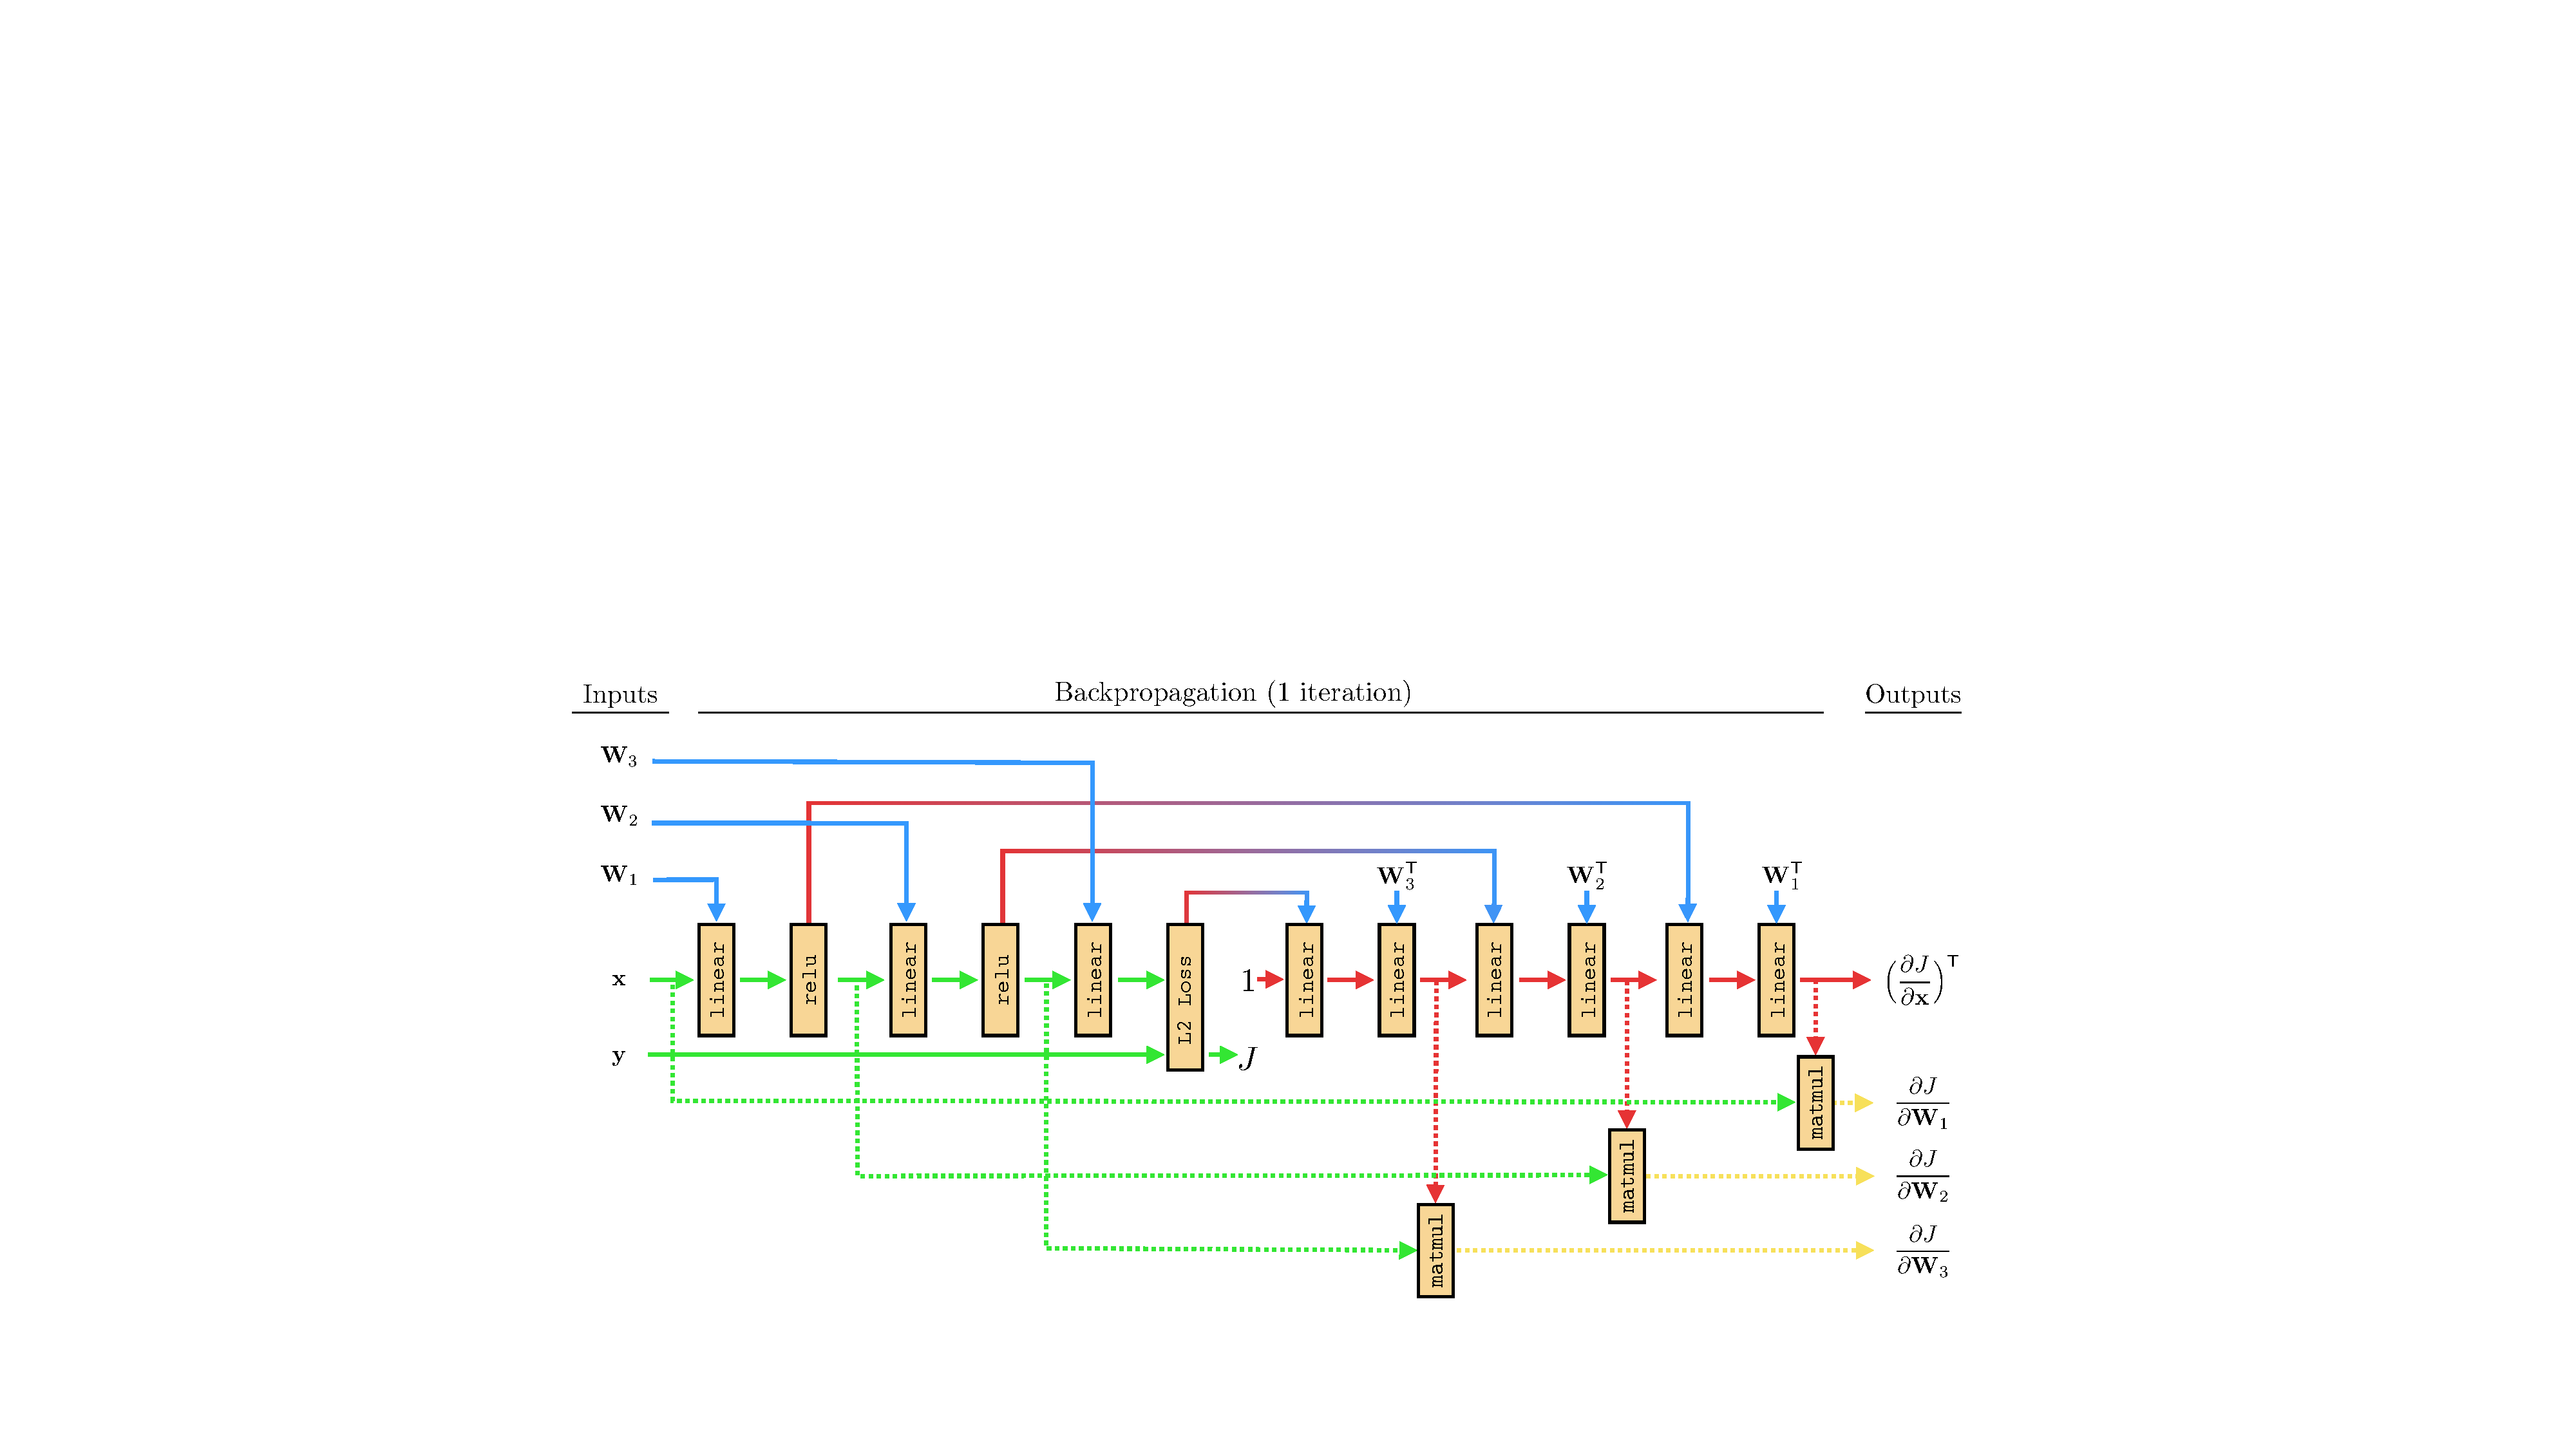
\includegraphics[width=1.0\linewidth]{./figures/backpropagation/backprop_as_neural_net.pdf}
    }
    \caption{The computation graph for backpropagation through a three-layer MLP. It's just another neural net! Solid lines are involved in computing data/activation gradients and dotted lines are involved in computing parameter gradients.\\ \hfill \break\raisebox{0.5mm}{\textcolor{comp_graph_param_bcolor}{\rule{4mm}{2pt}}} : params \texttt{forward}\\\raisebox{0.5mm}{\textcolor{backwardpropcolor_params}{\rule{4mm}{2pt}}} : params \texttt{backward}\\\raisebox{0.5mm}{\textcolor{forwardpropcolor}{\rule{4mm}{2pt}}} : data \texttt{forward}\\\raisebox{0.5mm}{\textcolor{backwardpropcolor}{\rule{4mm}{2pt}}} : data \texttt{backward}}
    \label{fig:backpropagation:backprop_as_neural_net}
\end{figure}

There are a few interesting things about this forward-backward network. One is that \textit{activations} from the \texttt{relu} layers get transformed to become \textit{parameters} of a \texttt{linear} layer of the backward network (see \eqn{\ref{eqn:backpropagation:pointwise_costgrad}}). There is a general term for this setup, where one neural net outputs values that parameterize another neural net; this is called a \index{Hypernetwork}\textbf{hypernetwork}~\cite{ha2016hypernetworks}. The forward network is a hypernetwork that parameterizes the backward network.

Another interesting property, which we already pointed out previously, is that the backward network only consists of linear layers. This is true no matter what the forward network consists of (even if it is not a conventional neural network but some arbitrary computation graph). The reason why this happens is because backprop implements the chain rule, and the chain rule is always a product of Jacobian \textit{matrices}. Since a Jacobian is a matrix, clearly it is a linear function. But more intuitively, you can think of each Jacobian as being a locally linear approximation to the loss surface; hence each can be represented with a linear layer.


\section{Backpropagation through DAGs: Branch and Merge}\label{sec:backpropagation:branch_and_merge}

So far we have only seen chain-like graphs, --[]--[]--[]$\rightarrow$. Can backprop handle other graphs? It turns out the answer is \textit{yes}. Presently we will consider \index{Directed acyclic graph}{\bf directed acyclic graphs} ({\bf DAGs}). In \chap{\ref{chapter:recurrent_neural_nets}}, we will see that neural nets can also include cycles and still be trained with variants of backprop (e.g., backprop through time).

In a DAG, nodes can have multiple inputs and multiple outputs. In fact, we have already seen several examples of such nodes in the preceding sections. For example, a linear layer can be thought of as having two inputs, $\xin$ and $\theta$, and one output $\xout$; or it can be thought of as having $N = |\xin| + |\theta|$ inputs and $M = |\xout|$ outputs, if we count up each dimension of the input and output vectors. So we have already seen DAG computation graphs.

However, to work with general DAGs, it helps to introduce two new special modules, which act to construct the topology of the graph. We will call these special operators \texttt{merge} and \texttt{branch} (\fig{\ref{fig:backpropagation:branch_and_merge}}).\marginnote{We only consider binary branching and merging here, but branching and merging $N$ ways can be done analogously or by repeating these operators.}[-1.8cm] %\texttt{Branch} takes data and makes two copies of it, sent to two different subsequent modules. \texttt{Merge} takes two input data vectors and concatenates them into a single output vector. 
% \begin{figure}[h]
%     \centering
%     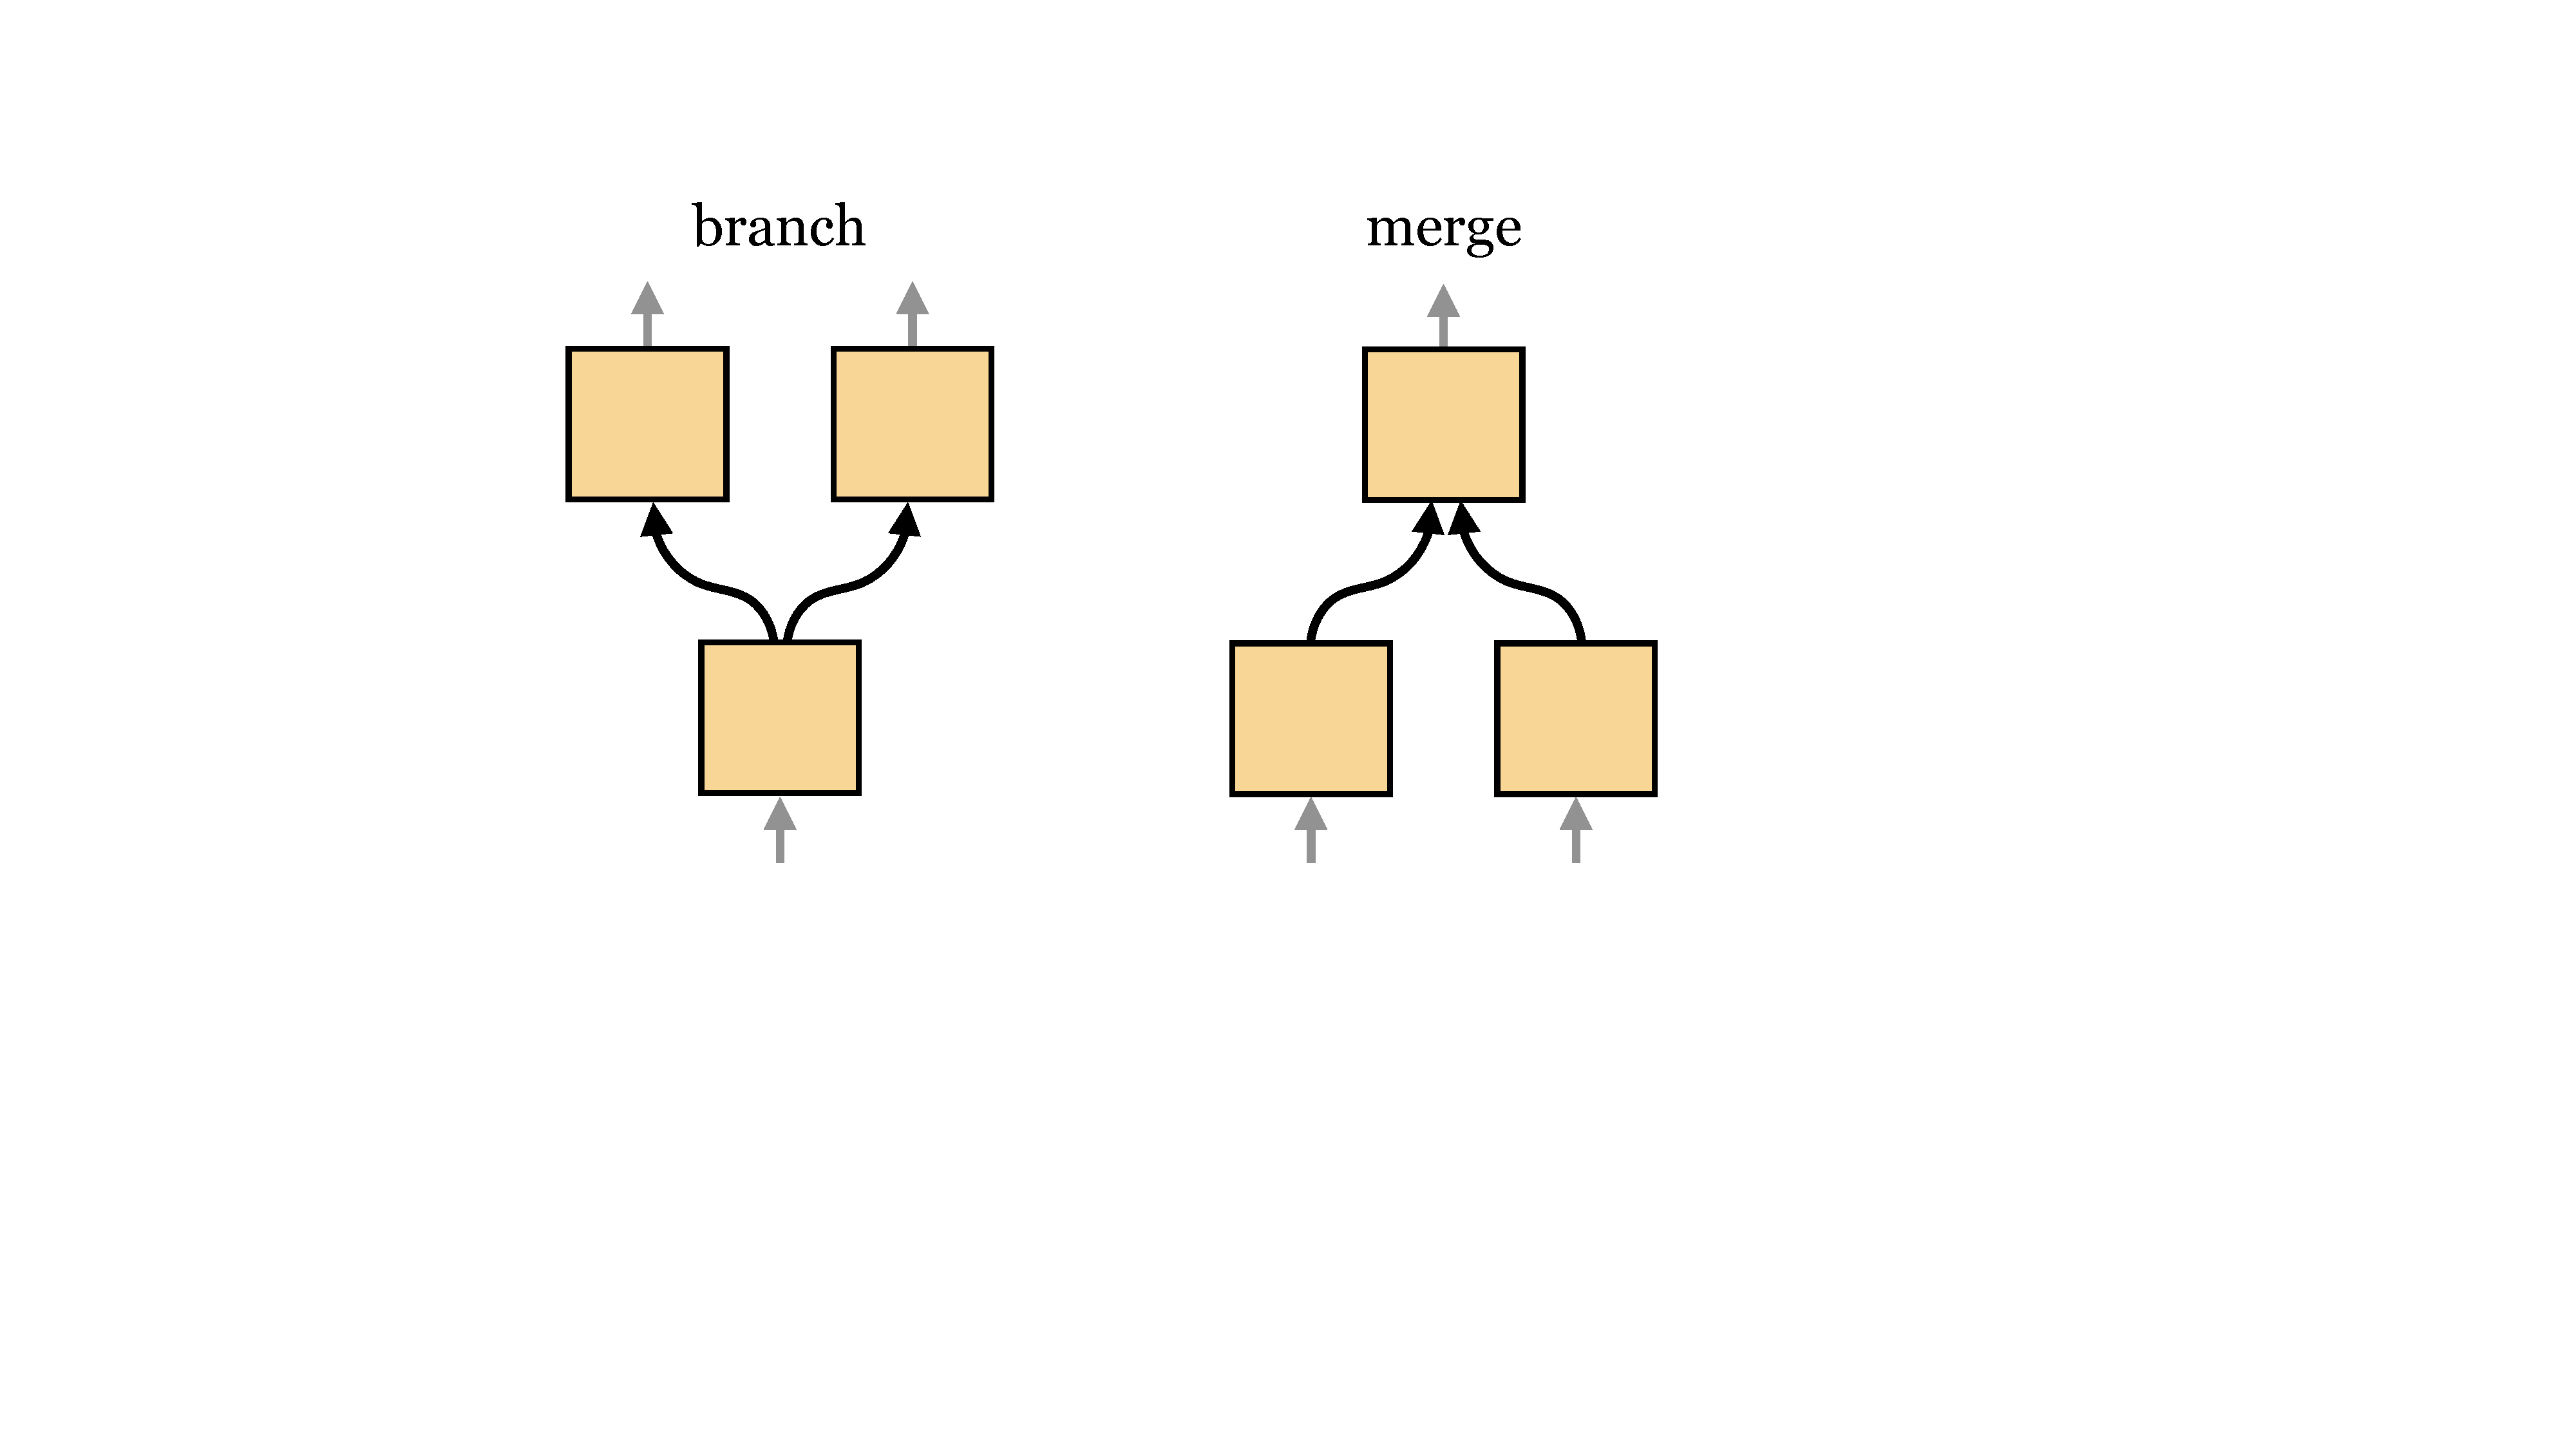
\includegraphics[width=0.42\linewidth]{./figures/backpropagation/branch_merge.pdf}
%     \label{fig:backprop_branch_merge}
% \end{figure}

\begin{figure}[h]
\def\layerwidth{1.5}
\centerline{
\begin{minipage}{0.33\linewidth}
\centering
\begin{tikzpicture}[
cblock/.style={
draw,
fill=comp_graph_node_bcolor,
rectangle, 
inner sep=1.5mm,
minimum width=\layerwidth*0.9 cm,
minimum height=\layerwidth*0.5*0.9 cm,
font=\footnotesize}]
%
\node (a) at (-0.2,-\layerwidth*0.5) {};
\node (b) at (-0.2,\layerwidth*0.5) {};
\node (c) at (\layerwidth*0.6,0) {};
\path [thick] [comp_graph_edge] (a) edge [out=0,in=180] (c);
\path [thick] [comp_graph_edge] (b) edge [out=0,in=180] (c);
%
\draw (\layerwidth*1,0) node [cblock] {\texttt{merge}};
\draw [thick] [comp_graph_edge] (\layerwidth*1.5,0) -- (\layerwidth*2,0);
%
\end{tikzpicture}
\end{minipage}
\begin{minipage}{0.33\linewidth}
\centering
\begin{tikzpicture}[
cblock/.style={
draw,
fill=comp_graph_node_bcolor,
rectangle, 
inner sep=1.5mm,
minimum width=\layerwidth*0.9 cm,
minimum height=\layerwidth*0.5*0.9 cm,
font=\footnotesize}]
%
\draw [thick] [comp_graph_edge] (0,0) -- (\layerwidth*0.5,0);
\draw (\layerwidth,0) node [cblock] {\texttt{branch}};
%
\node (a) at (\layerwidth*1.4,0) {};
\node (b) at (\layerwidth*2+0.2,-\layerwidth*0.5) {};
\path [thick] [comp_graph_edge] (a) edge [out=0,in=180] (b);
\node (c) at (\layerwidth*2+0.2,\layerwidth*0.5) {};
\path [thick] [comp_graph_edge] (a) edge [out=0,in=180] (c);
%
\end{tikzpicture}
\end{minipage}
}
\caption{The \texttt{merge} and \texttt{branch} layers.}
\label{fig:backpropagation:branch_and_merge}
\end{figure}

We define them mathematically as variable concatenation and copying, respectively:
\begin{align}
    \texttt{merge}(\xin^a, \xin^b) &\triangleq [\xin^a, \xin^b] \triangleq \xout\\
    \texttt{branch}(\xin) &\triangleq [\xin, \xin] \triangleq [\xout^a, \xout^b]
\end{align}
\marginnote{What if $\xin^a$ and $\xin^b$ are tensors, or other objects, with different shapes? Can we still concatenate them? The answer is yes. The shape of the data tensor has no impact on the math. We pick the shape just as a notational convenience; for example, it's natural to think about images as two-dimensional arrays.}[-1.2cm]
Here, $\texttt{merge}$ takes two inputs and concatenates them. This results in a new multidimensional variable. The backward pass equation is trivial. To compute the gradient of the cost with respect to $\xin^{a}$, that is, $\costgradin^a$, we have
\begin{align}
    \costgradin^{a} &= \costgradout \localgrad^{\mathbf{x}^a} = \frac{\partial J}{\partial \xout} \frac{\partial \xout}{\partial \xin^{a}}\\ %= \frac{\partial J}{\partial \mathbf{x}} \frac{\partial \texttt{merge}}{\partial \mathbf{x}^{a}}\\
    &= \costgradout \Big[\frac{\partial \xin^{a}}{\partial \xin^{a}}, \frac{\partial \xin^{b}}{\partial \xin^{a}}\Big]^\transpose\\
    &= \costgradout [1, 0]^\transpose
\end{align}
and likewise for $\costgradin^b$. That is, we just pick out the first half of the $\costgradout$ gradient vector for $\costgradin^a$ and the second half for $\costgradin^b$. There is really nothing new here. We already defined backpropagation for multidimensional variables above, and $\texttt{merge}$ is just an explicit way of constructing multidimensional variables.

%We already defined backprop for multidimensional inputs, and nothing is different here. The gradients propagated backwards are $\frac{\partial J}{\partial \mathbf{x}^{\prime}}$.

The \texttt{branch} operator is only slightly more complicated. In branching, we send \textit{copies} of the same output to multiple downstream nodes. Therefore, we have multiple gradients coming back to the $\texttt{branch}$ module, each from different downstream paths. So the inputs to this module on the backward pass are $\frac{\partial J}{\partial \xin^{a}}, \frac{\partial J}{\partial \xin^{b}}$, which we can write as the gradient vector $\costgradout = \frac{\partial J}{\partial [\xin^a, \xin^b]} = [\frac{\partial J}{\partial \xin^{a}}, \frac{\partial J}{\partial \xin^{b}}] = [\costgradout^a, \costgradout^b]$.  Let's compute the backward pass output:
\begin{align}
    \costgradin &= \costgradout \localgrad^{\mathbf{x}}\\
    &= [\costgradout^a, \costgradout^b] \frac{\partial [\xout^a, \xout^b]}{\partial \xin}\\
    &= [\costgradout^a, \costgradout^b] \frac{\partial [\xin, \xin]}{\partial \xin}\\
    &= [\costgradout^a, \costgradout^b][1, 1]^\transpose\\
    &= \costgradout^b + \costgradout^b
\end{align}
So, branching just sums both the gradients passed backward to it.
%Suppose our output is $\mathbf{x}^{l+1}$. Then, during backprop, we have multiple different versions of $\partial L \partial x$ being propagated back. How should resolve all these different versions? Consider the simple case where we have two output branches. 

Both $\texttt{merge}$ and $\texttt{branch}$ have no parameters, so there is no parameter gradient to define. Thus, we have fully specified the forward and backward behavior of these layers. The next diagrams summarize the behavior (\fig{\ref{fig:backpropagation:branch_and_merge_layers_backprop_diagram}}).
% \begin{figure}[h]
%     \centering
%     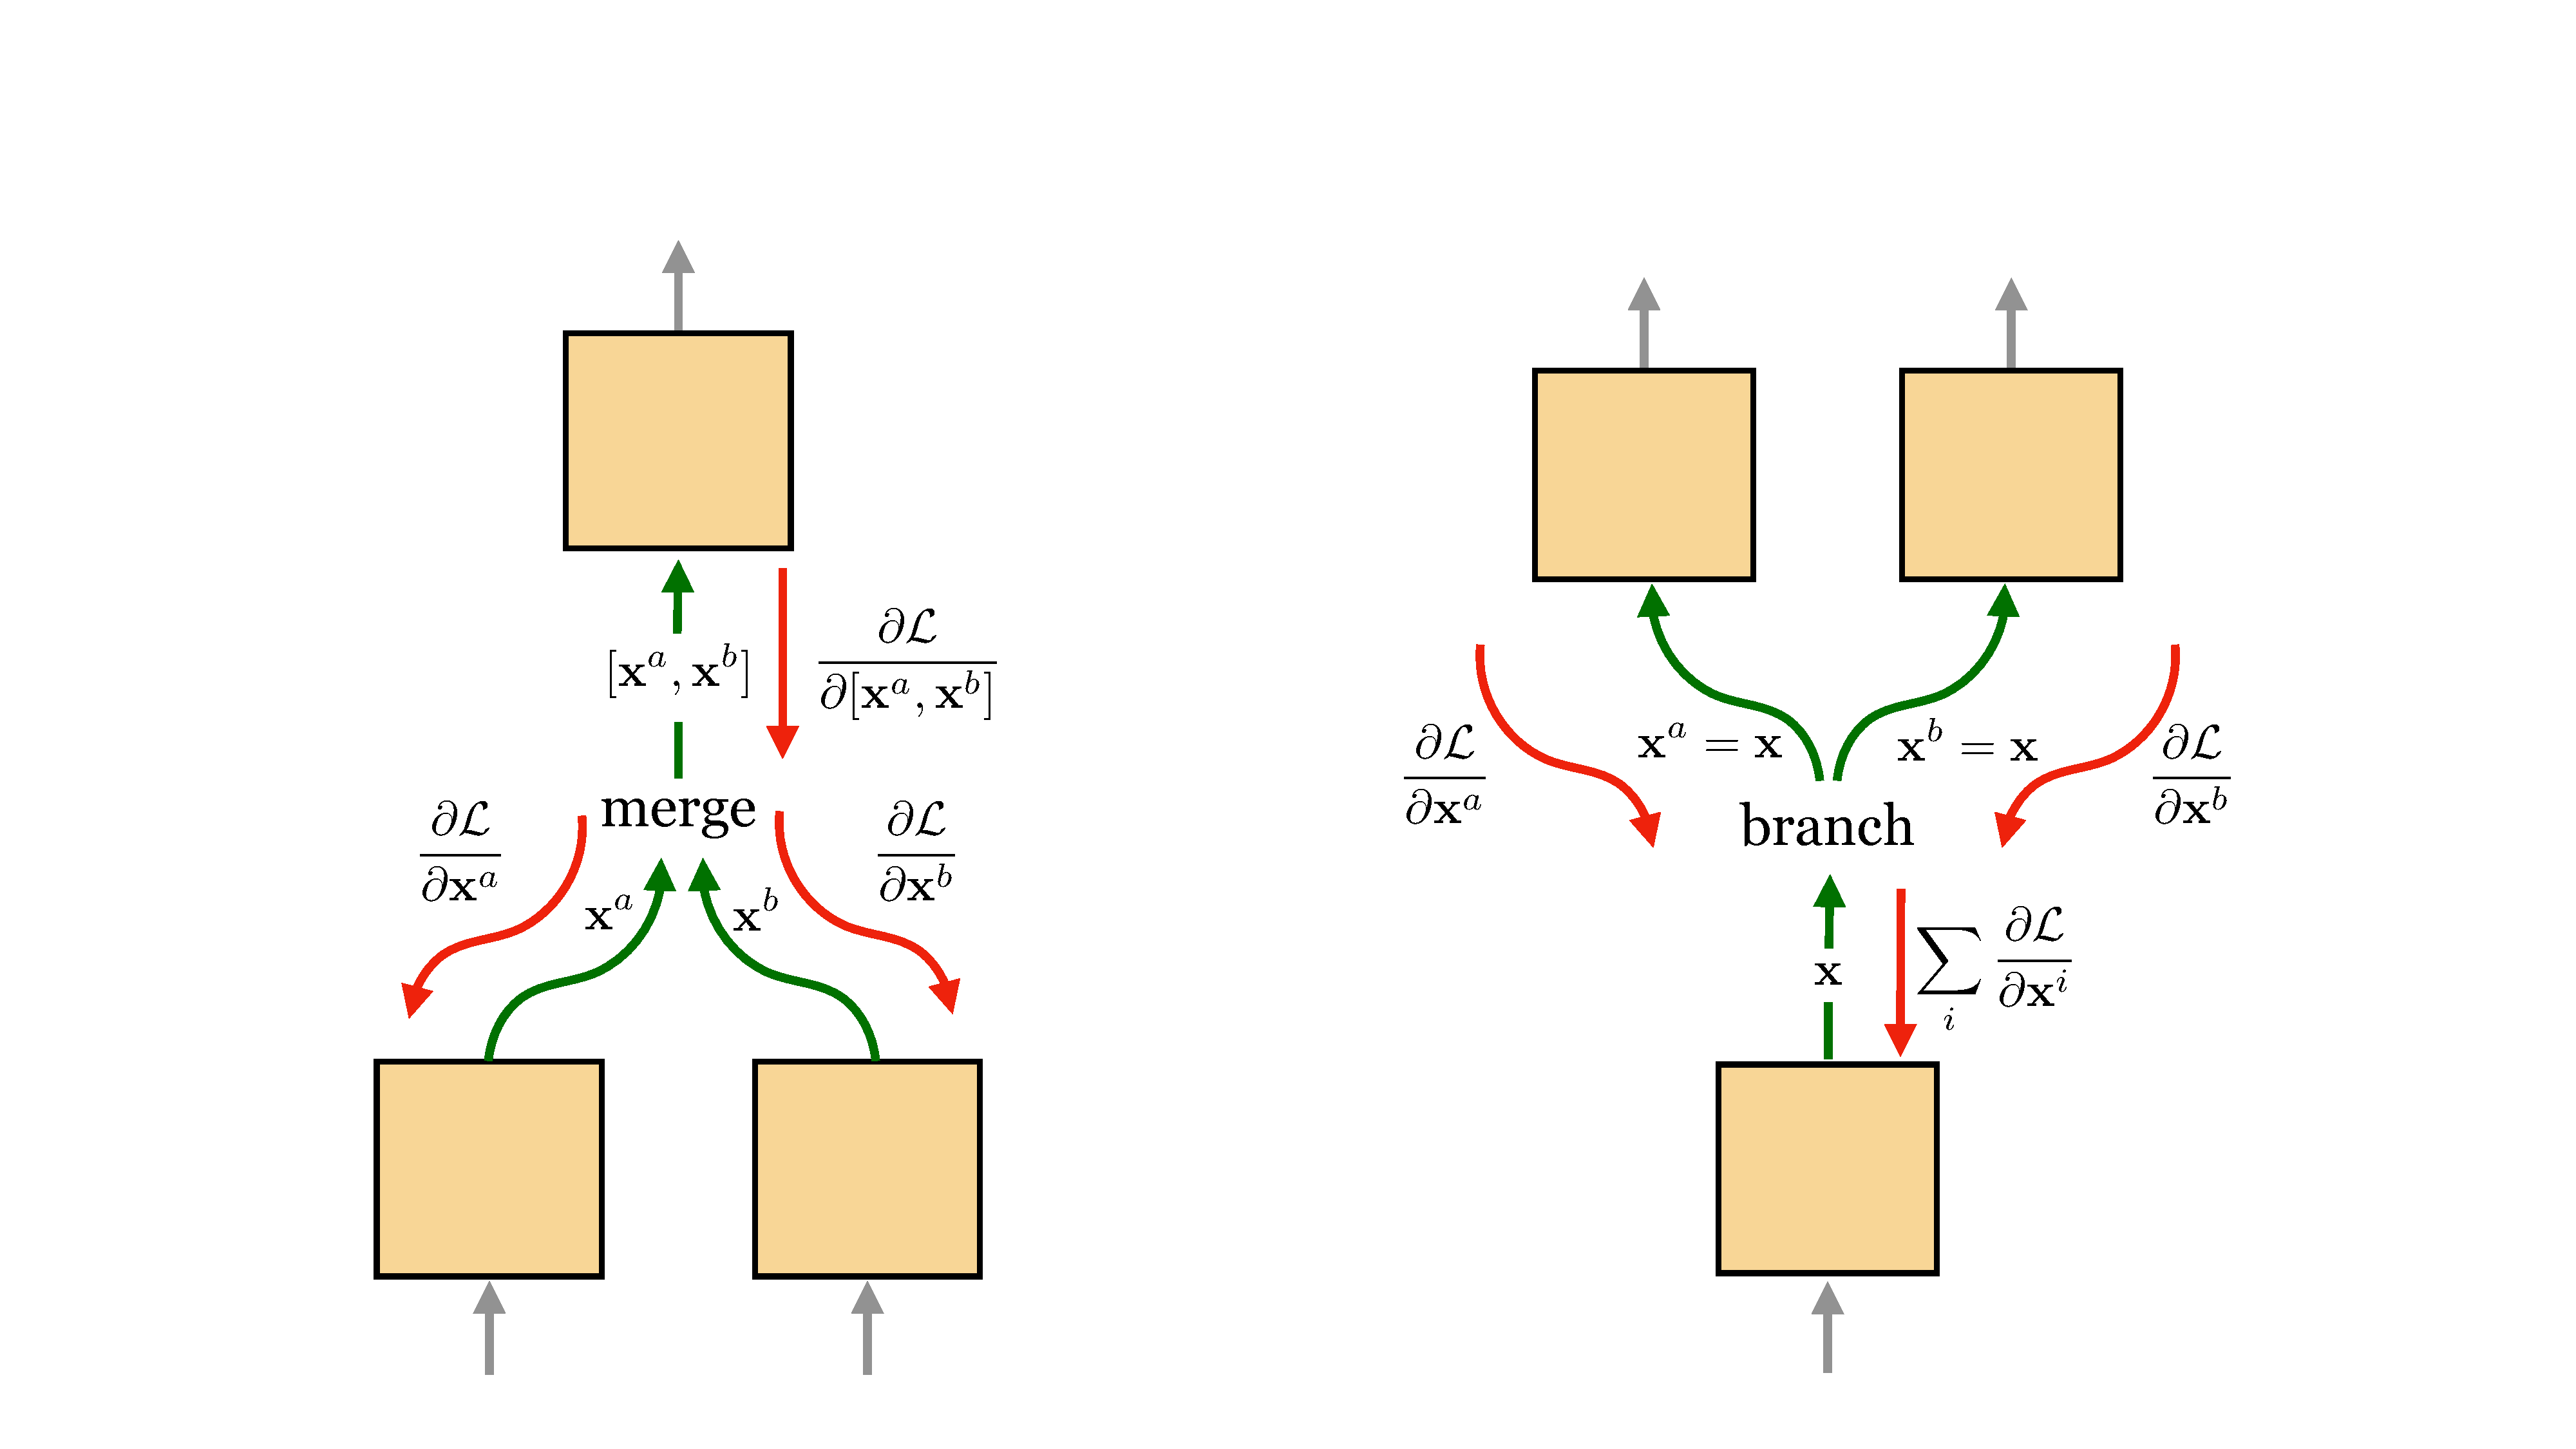
\includegraphics[width=0.75\linewidth]{./figures/backpropagation/branch_merge_gradient_diagrams.pdf}
%     \label{fig:backprop_branch_merge_gradient_diagrams}
% \end{figure}
\begin{figure}[h]
\centerline{
\begin{minipage}{0.48\linewidth}
\centering
\begin{tikzpicture}%[>=spaced latex]
%
\def\layerwidth{1.6}
%
\draw [thick] [comp_graph_edge_forward] (0.4,0.6) -- (\layerwidth*0.6,0.6);
\draw [thick] [comp_graph_edge_forward] (0.4,1.2) -- (\layerwidth*0.6,1.2);
\draw [thick] [comp_graph_edge_backward] (\layerwidth*0.6,0) -- (0.4,0);
\draw [thick] [comp_graph_edge_backward] (\layerwidth*0.6,-0.6) -- (0.4,-0.6);
\draw (\layerwidth*1.5,0.3) node [fill=comp_graph_node_bcolor,draw, inner sep=2mm, minimum height=2.6cm, minimum width=2.8cm] {};
\draw (\layerwidth*1.5,2.4) node {\textbf{merge layer}};
\draw (\layerwidth*1.5,2.0) node {\texttt{forward} and \texttt{backward}};
\draw (\layerwidth*1.5,0.9) node  {$\xout = [\xin^a, \xin^b]$};
\draw (\layerwidth*1.5,0) node  {$\costgradin^a = \costgradout [1, 0]^\transpose$};
\draw (\layerwidth*1.5,-0.6) node  {$\costgradin^b = \costgradout [0, 1]^\transpose$};
\draw [thick] [comp_graph_edge_forward] (\layerwidth*2.4,0.9) -- (\layerwidth*2.75,0.9);
\draw [thick] [comp_graph_edge_backward] (\layerwidth*2.8,-0.3) -- (\layerwidth*2.4,-0.3);
%
\draw (-0.1,1.2) node [fill=comp_graph_data_bcolor] {$\xin^a$};
\draw (-0.1,0.6) node [fill=comp_graph_data_bcolor] {$\xin^b$};
\draw (0,0) node [fill=comp_graph_data_bcolor] {$\costgradin^a$};
\draw (0,-0.6) node [fill=comp_graph_data_bcolor] {$\costgradin^b$};
\draw (\layerwidth*3,-0.3) node [fill=comp_graph_data_bcolor] {$\costgradout$};
\draw (\layerwidth*3,0.9) node [fill=comp_graph_data_bcolor] {$\xout$};
%
\end{tikzpicture}
\end{minipage}
\begin{minipage}{0.48\linewidth}
\centering
\begin{tikzpicture}%[>=spaced latex]
%
\def\layerwidth{1.6}
%
\draw [thick] [comp_graph_edge_forward] (0.4,0.9) -- (\layerwidth*0.6,0.9);
\draw [thick] [comp_graph_edge_backward] (\layerwidth*0.6,-0.3) -- (0.4,-0.3);
\draw (\layerwidth*1.5,0.3) node [fill=comp_graph_node_bcolor,draw, inner sep=2mm, minimum height=2.6cm, minimum width=2.8cm] {};
\draw (\layerwidth*1.5,2.4) node {\textbf{branch layer}};
\draw (\layerwidth*1.5,2.0) node {\texttt{forward} and \texttt{backward}};
\draw (\layerwidth*1.5,0.6) node  {$\xout^a = \xin$};
\draw (\layerwidth*1.5,1.2) node  {$\xout^b = \xin$};
\draw (\layerwidth*1.5,-0.3) node  {$\costgradin = \costgradout^a + \costgradout^b$};
\draw [thick] [comp_graph_edge_forward] (\layerwidth*2.4,0.6) -- (\layerwidth*2.75,0.6);
\draw [thick] [comp_graph_edge_forward] (\layerwidth*2.4,1.2) -- (\layerwidth*2.75,1.2);
\draw [thick] [comp_graph_edge_backward] (\layerwidth*2.8,0) -- (\layerwidth*2.4,0);
\draw [thick] [comp_graph_edge_backward] (\layerwidth*2.8,-0.6) -- (\layerwidth*2.4,-0.6);
%
\draw (-0.1,0.9) node [fill=comp_graph_data_bcolor] {$\xin$};
\draw (0,-0.3) node [fill=comp_graph_data_bcolor] {$\costgradin$};
\draw (\layerwidth*3,0) node [fill=comp_graph_data_bcolor] {$\costgradout^a$};
\draw (\layerwidth*3,-0.6) node [fill=comp_graph_data_bcolor] {$\costgradout^b$};
\draw (\layerwidth*3,1.2) node [fill=comp_graph_data_bcolor] {$\xout^a$};
\draw (\layerwidth*3,0.6) node [fill=comp_graph_data_bcolor] {$\xout^b$};
%
\end{tikzpicture}
\end{minipage}
}
\caption{Merge and branch layers \texttt{forward} and \texttt{backward}.}
\label{fig:backpropagation:branch_and_merge_layers_backprop_diagram}
\end{figure}

With \texttt{merge} and \texttt{branch}, we can construct any DAG computation graph by simply inserting these layers wherever we want a layer to have multiple inputs or multiple outputs. An example is given in \fig{\ref{fig:backpropagation:backprop_DAG}}.
\begin{figure}[h]
    \centerline{
    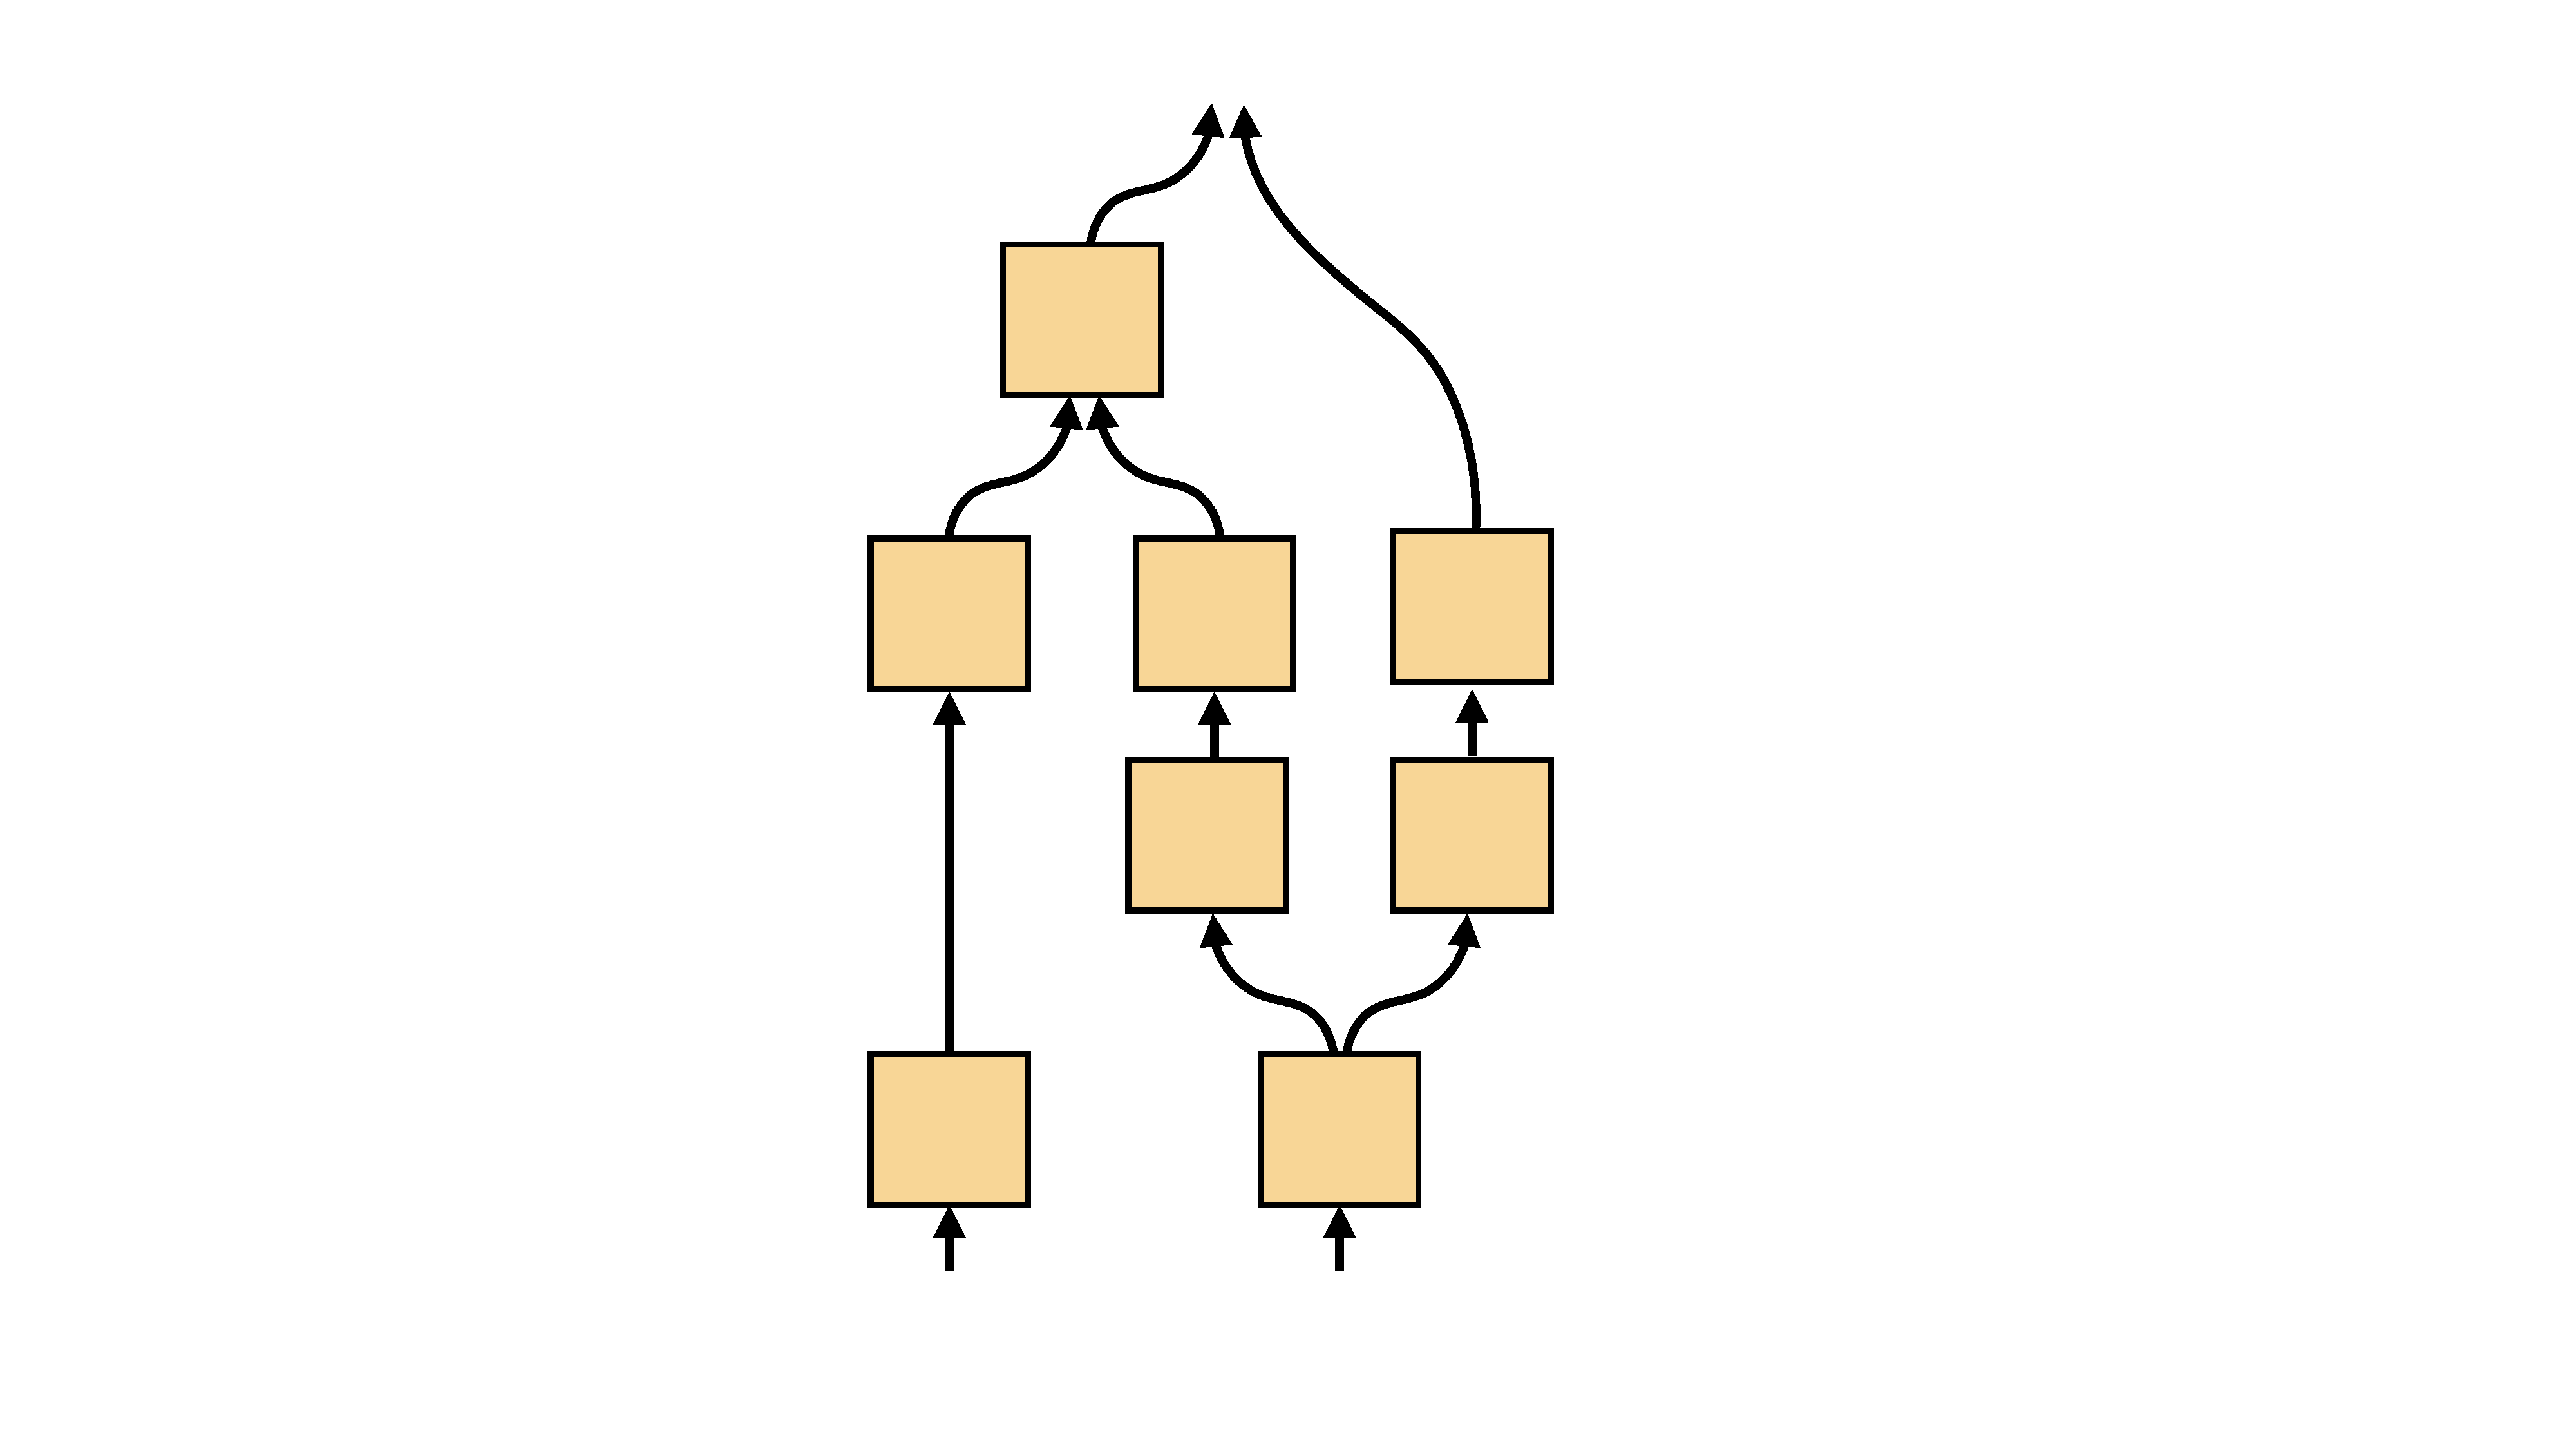
\includegraphics[width=0.25\linewidth, angle=-90]{./figures/backpropagation/DAG.pdf}
    }
    \caption{An example of a DAG computation graph that we can construct, and do backpropagation through, with the tools defined previously.}
    \label{fig:backpropagation:backprop_DAG}
\end{figure}

\section{Parameter Sharing}

\index{Parameter sharing}\textbf{Parameter sharing} consists of a single parameter being sent as input to multiple different layers. We can consider this as a branching operation, as shown in \fig{\ref{fig:backpropagation:parameter_sharing}}.
\begin{figure}[h]
\centerline{
\def\layerwidth{1.5}
\begin{tikzpicture}[
cblock/.style={
draw,
fill=comp_graph_node_bcolor,
rectangle, 
inner sep=1.5mm,
minimum width=\layerwidth*0.5 cm,
minimum height=\layerwidth*0.5*0.9 cm,
font=\footnotesize}]
%
\draw [thick] [comp_graph_edge] (0,0) -- (\layerwidth*0.5,0);
\draw (\layerwidth,0) node [cblock] {\texttt{branch}};
%
\node (a) at (\layerwidth*1.4,0) {};
\node (b) at (\layerwidth*2+0.2,-\layerwidth*0.5) {};
\path [thick] [comp_graph_edge] (a) edge [out=0,in=180] (b);
\node (c) at (\layerwidth*2+0.2,\layerwidth*0.5) {};
\path [thick] [comp_graph_edge] (a) edge [out=0,in=180] (c);
%
\draw (-0.2,0) node [fill=comp_graph_param_bcolor] {$\theta$};
\draw (\layerwidth*2+0.4,-\layerwidth*0.5) node [fill=white] {$\theta^a$};
\draw (\layerwidth*2+0.4,\layerwidth*0.5) node [fill=white] {$\theta^b$};
%
\draw (\layerwidth*3,-\layerwidth*0.5) node [cblock, minimum height=\layerwidth*0.5*1.3 cm] {};
\draw (\layerwidth*3,\layerwidth*0.5) node [cblock, minimum height=\layerwidth*0.5*1.3 cm] {};
\draw [thick] [comp_graph_edge] (\layerwidth*2+0.6,-\layerwidth*0.5) -- (\layerwidth*2.75,-\layerwidth*0.5);
\draw [thick] [comp_graph_edge] (\layerwidth*2+0.6,\layerwidth*0.5) -- (\layerwidth*2.75,\layerwidth*0.5);
\draw [thick] [comp_graph_edge] (\layerwidth*3.25,-\layerwidth*0.5) -- (\layerwidth*3.75,-\layerwidth*0.5);
\draw [thick] [comp_graph_edge] (\layerwidth*3.25,\layerwidth*0.5) -- (\layerwidth*3.75,\layerwidth*0.5);
%
\draw (\layerwidth*2+0.3,-\layerwidth*0.75) node [fill=white] {$\cdots$};
\draw (\layerwidth*2+0.3,\layerwidth*0.75) node [fill=white] {$\cdots$};
\draw [thick] [comp_graph_edge] (\layerwidth*2+0.6,-\layerwidth*0.75) -- (\layerwidth*2.75,-\layerwidth*0.75);
\draw [thick] [comp_graph_edge] (\layerwidth*2+0.6,\layerwidth*0.75) -- (\layerwidth*2.75,\layerwidth*0.75);
%
\end{tikzpicture}
}
\caption{Parameter sharing is equivalent to branching a parameter in the computation graph.}
\label{fig:backpropagation:parameter_sharing}
\end{figure}

Then, from the previous section, it is clear that gradients summate for shared parameters. Let $\{\theta^i\}^N_{i=1}$ be a set of variables that are all copies of one free parameter {\setlength{\fboxsep}{2pt}\colorbox{comp_graph_param_bcolor}{$\theta$}}. Then, 
\begin{align}
    \frac{\partial J}{\partial \theta} = \sum_i \frac{\partial J}{\partial \theta^i}
\end{align}\marginnote{Neural net layers that have their parameters shared in this way are sometimes said to use \index{Weight tying}\textbf{tied weights}.}[-1.8cm]

% \section{Backprop is a beautiful tool}

% Backprop is often presented as just a way to compute the parameter gradient for neural nets. But it is actually a very general tool that can be used for many other purposes. In this chapter we presented it as a way to efficiently compute gradients for any variable in a computation graph. Here are some fun things you can do with backprop beyound just using it for fitting neural net parameters.

\section{Backpropagation to the Data}

Backpropagation does not distinguish between parameters and data — it treats both as generic inputs to parameterless modules. Therefore, we can use backprop to optimize data inputs to the graph just like we can use backprop to optimize parameter inputs to the graph.

To see this, it helps to think about just the inputs and outputs to the full computation graph. In the forward direction, the inputs are the data and parameter settings and the output is the loss. In the backward direction, the input is the number 1 and the outputs are the are gradients of the loss with respect to the data and parameters. The full computation graph, for a learning problem using neural net $F = f_L \circ \cdots \circ f_1$ and loss function $\mathcal{L}$, is $\mathcal{L}(F(\mathbf{x}_0), \mathbf{y}, \theta) \triangleq J(\mathbf{x}_0, \mathbf{y}, \theta)$. This function can itself be thought of as a single computation block, with inputs and outputs as specified previously (\fig{\ref{fig:backpropagation:J_forward_backward_blocks}}).
\marginnote{In Pytorch you can only set \textit{input} variables as optimization targets -- these are called the \textit{leaves} of the computation graph since, on the backward pass, they have no children. All the other variables are completely determined by the values of the input variables — they are not \textit{free} variables.}[-5cm]
\begin{figure}[h]
\centerline{
\begin{minipage}{.45\textwidth}
\begin{tikzpicture}%[>=spaced latex]
%
\def\layerwidth{1.9}
%
\draw [thick] [comp_graph_edge] (\layerwidth*0.6,-0.35) -- (\layerwidth,-0.35);
\draw [thick] (\layerwidth*0.6,-0.75) -- (\layerwidth*0.6,-0.35);
\draw [thick] [comp_graph_edge] (\layerwidth*0.5,0) -- (\layerwidth,0);
\draw (\layerwidth*1.5,0) node [fill=comp_graph_node_bcolor,draw, inner sep=2mm, minimum height=1.3cm] {$J(\mathbf{x}_0, \mathbf{y}, \theta)$};
\draw [thick] [comp_graph_edge] (\layerwidth*2,0) -- (\layerwidth*2.4,0);
%
\draw (\layerwidth*0.6,-0.95) node [fill=comp_graph_param_bcolor] {$\theta$};
\draw (\layerwidth*0.2,0) node [fill=forwardpropcolor] {$\mathbf{x}_0, \mathbf{y}$};
\draw (\layerwidth*2.55,0) node [fill=comp_graph_data_bcolor] {$J$};
%
\draw (\layerwidth*1.5,1.0) node {$J$ \texttt{Forward}};
%
\end{tikzpicture}
\end{minipage}
\begin{minipage}{.45\textwidth}
\begin{tikzpicture}%[>=spaced latex]
%
\def\layerwidth{1.9}
%
\draw [thick] (\layerwidth,-0.35) -- (\layerwidth*0.6,-0.35);
\draw [thick] [comp_graph_edge](\layerwidth*0.6,-0.35) -- (\layerwidth*0.6,-0.75);
\draw [thick] [comp_graph_edge] (\layerwidth,0) -- (\layerwidth*0.55,0);
\draw (\layerwidth*1.5,0) node [fill=comp_graph_node_bcolor,draw, inner sep=2mm, minimum height=1.3cm] {$J^{\prime}(\mathbf{x}_0, \mathbf{y}, \theta)$};
\draw [thick] [comp_graph_edge] (\layerwidth*2.4,0) -- (\layerwidth*2.05,0);
%
\draw (\layerwidth*0.6,-1.1) node [fill=backwardpropcolor_params, thick] {$\frac{\partial J}{\partial \theta}$};
\draw (\layerwidth*0.2,0) node [fill=backwardpropcolor] {$\frac{\partial J}{\partial \mathbf{x}_0}, \frac{\partial J}{\partial \mathbf{y}}$};
\draw (\layerwidth*2.55,0) node [fill=comp_graph_data_bcolor] {$1$};
%
\draw (\layerwidth*1.5,1.0) node {$J$ \texttt{Backward}};
%
\end{tikzpicture}
\end{minipage}
}
\caption{Full forward and backward passes for a learning problem $\min J(\mathbf{x}_0,\mathbf{y},\theta)$, collapsed into a single computation block.}
\label{fig:backpropagation:J_forward_backward_blocks}
\end{figure}

From this diagram, it should be clear that data inputs and parameter inputs play symmetric roles. Just as we can optimize parameters to minimize the loss, by descending the parameter gradient given by \texttt{backward}, we can also optimize input data to minimize the loss by descending the data gradient.

This can be useful for lots of different applications. One example is visualizing the input image that most activates a given neuron we are probing in a neural net. To do this, we define $J$ to be the \textit{negative} of the value of the neuron we are probing\footnote{It is negative so that minimizing the loss maximizes the activation.}, that is, $J(\mathbf{x}_0,\theta) = -x_{l}[i]$ if we are interested in the $i$-th neuron on layer $l$ (notice $\mathbf{y}$ is not used for this problem). We show an example of this in \fig{\ref{fig:backpropagation:backprop_to_the_data_example}} below, where we used backprop to find the input image that most activates a node in the computation graph that scores whether or not an image is ``a photo of a cat.'' Do you see cat-like stuff in the optimized image? What does this tell you about how the network is working?
\begin{figure}[h!]
    \centerline{
    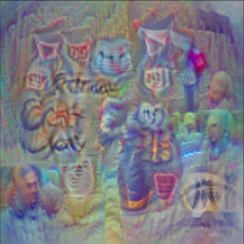
\includegraphics[width=.45\linewidth]{./figures/backpropagation/backprop_to_the_data_example.png}
    }
    \caption{Visualizing the optimal image of a cat according to a particular neural net. The net we used is called Contrastive Language-Image Pre-Training (CLIP)~\cite{radford2021learning} and here we found the image that maximizes a node in CLIP's computation graph that measures how much the image matches the text ``a photo of a cat.'' In \chap{\ref{chapter:VLMs}} we will cover exactly how the CLIP model works in more detail.}
    \label{fig:backpropagation:backprop_to_the_data_example}
\end{figure}

\marginnote{Visualizations like this are a useful way to figure out what visual features a given neuron is sensitive to. Researchers often combine this visualization method with a natural image prior in order to find an image that not only strongly activates the neuron in question but also looks like a natural photograph (e.g., \cite{olah2017feature}).}[-0.6cm]

% \subsection{Backprop through backprop}
% \reviewcomment{Unfinished}
% In Section \ref{section:backpropagation:backprop_as_neural_net}, we learned that the entire backprop algorithm can be implemented as a ``forward-backward" neural network. You may have wondered: what if we then apply backprop again to \textit{that} neural net?

% It turns out that indeed we can do this, and it has several interesting applications. To illustrate, we will describe a method called MAML~\cite{MAML}, whose goal is to learn a parameter vector that is just a few gradient steps away from a good solution.

% Writing this goal in math, we have:
% \begin{align}
%     \argmin_{\theta_0} GD_{\theta}(\mathcal{L}(f_{\theta}(\mathbf{x}_0),\mathbf{y})
% \end{align}
% where \texttt{GD} is a gradient descent algorithm.

% First, let our ``forward-backward" be:
% \begin{align}
%     [\frac{\partial J}{\partial \mathbf{x}_0}, \frac{\partial J}{\partial \theta}] = \texttt{backward}(\texttt{forward}(\mathbf{x}_0, \mathbf{y}, \theta)) \triangleq
% \end{align}
% Now we need a cost function 

% MAML
% What if we want to find the initial image that, after one step of backprop to optimize the data, will get the best score. This is like a proto-image that can be easily turned into an image of each of our classes.

% \subsection{Backprop for nondifferentiable layers}
% \reviewcomment{Unfinished}

% ES

\section{Concluding Remarks}
Backprop is often presented as a method just for training neural networks, but it is actually a much more general tool than that. Backprop is an efficient way to find partial derivatives in computation graphs. It is general to a large family of computation graphs and can be used not just for learning parameters but also for optimizing data. %It is a beautiful algorithm and we will encounter it many times in this book.